\documentclass[10pt]{article}
\usepackage{amsmath, amssymb}
\usepackage{xparse}
\usepackage{graphicx}

\begin{document}
\tableofcontents
\section{Introduction}

Script of the Reinforcment Learning Course by David Silver
as uploaded on YouTube from 2015

written by Alex Liebenau \newline
created in November 2022 \newline
free to use \newline
\newpage
\section{Lecture two: Markov Decision Process (MDP)}
\subsection{Markov Process}

The current state characterises the process -> we are told the state --> environment is fully observable\newline

Almost all RL problems can be formalised as MDPs\newline
--> Optimal control primarily deals with continious MDPs\newline
--> Any partially observable problems can be converted into MDPs\newline
--> Bandits are MDPs with one state\newline

"The future is independent of the past given the present"

\begin{equation}
	\mathbb{P} \: [S_{t+1}\; | \; S_{t}] \; = \; \mathbb{P} \: [S_{t+1} \; | \; S_{1}, \ldots , S_{t}]
\end{equation}


What happens next only depends on what happend on the state before - you can throw away anything else.\newline

For a Markov state \textit{s} and successor state \textit{s'}, the \textit{state transition probability} is defined as

\begin{equation}
\mathcal{P}_{ss'} \; = \; \mathbb{P}\:[S_{t+1}\:=\:\textit{s'}\; | \; S_{t}\:=\:\textit{s}]
\end{equation}

State transition matrix $\rho$ defines transition probabilites from all states \textit{s} to all successor states \textit{s'}.

\begin{equation}
\mathcal{P} \; = \; from 
\stackrel{\mbox{$to$}}{\begin{pmatrix}
\mathcal{P}_{11} & \ldots & \mathcal{P}_{1n} \\
\vdots & & \\
\mathcal{P}_{n1} & \ldots & \mathcal{P}_{nn} \\
\end{pmatrix}}
\end{equation}

Each row of the matrix sums to 1! \newline
A Markov process is a memoryless random process, i.e. a sequence of random states, $S_{1}, \: S_{2}, \: \ldots$ with the Markov propoerty. It is defined as a tuple $\langle \mathcal{S}, \: \mathcal{P} \rangle$.
\begin{itemize}
\item S is a (finite) set of states
\item $\mathcal{P}$ is a state transition probability matrix
\end{itemize}

\subsection{Markov Reward process (MRP)}

The Markov Reward Process is defined as a tuple $\langle \mathcal{S}, \: \mathcal{P}, \: \mathcal{R}, \: \gamma \rangle$.
\begin{itemize}
\item $\mathcal{S}$ is a (finite) set of states
\item $\mathcal{P}$ is a state transition probability matrix
\item $\mathcal{R}$ is a reward function, $\mathcal{R}_{s} \: = \: \mathbb{E}[R_{t+1} \: | \: S_{t} = s]$
\item $\gamma$ is a discount factor, $\gamma \in [0,1]$
\end{itemize}

The \textit{return} $\mathcal{G}_{t}$ is the total discounted reward from time-step \textit{t}.

\begin{equation}
\mathcal{G}_{t} \; = \; R_{t+1} \; + \; \gamma R_{t+2} \; + \; \ldots \; = \;  \sum_{k=0}^{\infty} \;\gamma^{k} \: R_{t+k+1} 
\label{eq:g_t}
\end{equation}

\begin{itemize}
\item The discount $\gamma$ is the present value of future rewards - the closer $\gamma$ is to zero, the less are later rewards accounted (e.g. more 'short-sighted').
\item The value of receiving reward $\mathcal{R}$ after $k+1$ time-steps is $ \gamma^{k} R$.
\end{itemize}

\subsubsection*{Why discount?}
\begin{itemize}
\item Unless you really trust your model and believe that everything turns out as planned, you need to discount in deviations - Uncertainty about the future may not be fully represented
\item Mathematically convenient to discount rewards, avoids infinite returns
\item If the reward is financial, immediate rewards may earn more interest than delayed rewards
\item Animal/human behaviour shows preference for immediate reward
\item It is sometimes possible to use \textit{undiscounted} Markov reward process (i.e. $\gamma = 1$), e.g. if all sequences terminate.
\end{itemize}

\subsubsection*{The value function}

The value function \textit{v(s)} gives the long-term value of state s. It defines the expected return in a MRP starting from state \textit{s}:

\begin{equation}
v(s) \; = \; \mathbb{E}\;[G_{t} \; | \; S_{t} \; = \; s]
\end{equation}

The value function can be decomposed into two parts:

\begin{itemize}
\item immediate reward $R+1$
\item discounted value of successor state $\gamma v(S_{t+1})$
\end{itemize}

This resolves into the \textbf{Bellman equation for MRPs}:
\begin{equation}
v(s) \; = \; \mathbb{E}\;[G_{t} \; | \; S_{t} \; = \; s] \; = \; \mathbb{E}\;[R_{t+1} \; + \; \gamma v(S_{t+1}) \; | \; S_{t} \; = \; s]
\end{equation}

By averaging all possible outcomes we get
\begin{equation}
v(s) \; = \; \mathcal{R}_{s} \; + \; \gamma \: \sum_{s' \in \mathcal{S}} \mathcal{P}_{ss'}\:v(s')
 \label{eq:averaging_mrp}
\end{equation}

The Bellman  equation can be concisely using matrices, where $v$ is a column vector with one entry per state

\begin{equation}
v \; = \; \mathcal{R} \; + \; \gamma \: \mathcal{P} \: v \quad \rightarrow \quad
\begin{pmatrix}
v(1) \\ \vdots \\ v(n) \end{pmatrix} \; = \; \begin{pmatrix}
\mathcal{R}_{1} \\ \vdots \\ \mathcal{R}_{n} \end{pmatrix} \; + \; \gamma \; \begin{pmatrix}
\mathcal{P}_{11} & \ldots & \mathcal{P}_{1n} \\
\vdots & & \\
\mathcal{P}_{n1} & \ldots & \mathcal{P}_{nn} \\ \end{pmatrix} \; \begin{pmatrix}
v(1) \\ \vdots \\ v(n) \end{pmatrix} \label{eq:mrp_matrix}
\end{equation} 

The Bellman equation is linear. It can be solved directly by $v = (I - \gamma \mathcal{P})^{-1} \mathcal{R}$.

\begin{itemize}
\item The Computational complexity is O($n^{3}$) for \textit{n} states.
\item Direct solution only possible for small MRPs
\item Iterative methods for large MRPs, e.g. Dynamic programming, Monte-Carlo evaluation, Temporal-Difference learning
\end{itemize}

\subsection{Markov Decision Process (MDP)}
A MDP is a MRP with decisions. It is an \textit{environment} in which all states are Markov. \newline
A MDP is a tuple $\langle \mathcal{S, A, P, R,} \gamma \rangle$.

\begin{itemize}
\item $\mathcal{S}$ is a (finite) set of states
\item $\mathcal{A}$ is a (finite) set of actions
\item $\mathcal{P}$ is a state transition probability matrix \newline
$\mathcal{P}_{ss'}^{a} \; = \; \mathbb{P}\:[S_{t+1}\:=\:\textit{s'}\; | \; S_{t}\:=\:\textit{s}, \; A_{t}\:=\:\textit{a}]$
\item $\mathcal{R}$ is a reward function, $\mathcal{R}_{s}^{a}  \: = \: \mathbb{E}[R_{t+1} \: | \: S_{t} = s, \; A_{t}\:=\:\textit{a}]$
\item $\gamma$ is a discount factor, $\gamma \in [0,1]$
\end{itemize}

A policy $\pi$ is a distribution over actions given states. It fully defines the behaviour of an agent.
\begin{equation}
\pi(a|s) \; = \; \mathbb{P}\:[\:\: S_{t} = s, \; A_{t}\:=\:\textit{a}\:]
\end{equation}

In an MDP, the policies depend on the current state (not the history). Policies are stationary: $A_{t} = \pi ( \dot | S_{t} ), \forall t > 0$ \newline

Given an MDP $\mathcal{M} = \langle \mathcal{S, A, P, R,} \gamma \rangle$ and a policy $\pi$:
\begin{itemize}
\item The state sequence $S_{1}, S_{2}, \ldots$ is a Markov process $\langle \mathcal{S, P^{\pi}} \rangle$
\item The state and reward sequence $S_{1}, ,R_{2}, S_{2}, \ldots$ is a Markov reward process $\langle \mathcal{S}, \: \mathcal{P}, \: \mathcal{R}, \: \gamma \rangle$ where
\begin{equation}
\mathcal{P}_{s,s'}^{\pi} \; = \; \sum_{a \in \mathcal{A}} \; \pi (a|s)\: \mathcal{P}_{s,s'}^{a} \qquad
\mathcal{R}_{s}^{\pi} \; = \; \sum_{a \in \mathcal{A}} \; \pi (a|s)\: \mathcal{R}_{s}^{a} 
\end{equation}
\end{itemize}

The \textit{state-value function} $v_{\pi}(s)$ of an MDP is the expected return starting from state \textit{s}, and then following policy $\pi$:
\begin{equation}
v_{\pi}(s) \; = \; \mathbb{E}_{\pi} [ G_{t} \: | \: S_{t} \: = \: s] 
\end{equation}

The \textit{action-value function} $q_{\pi}(s, a)$ of an MDP is the expected return starting from state \textit{s}, taking action \textit{a}, and then following policy $\pi$:
\begin{equation}
q_{\pi}(s,a) \; = \; \mathbb{E}_{\pi} [ G_{t} \: | \: S_{t} \: = \: s, \: A_{t} \: = \: a] 
\end{equation}

The state-value and action-value functions can again be decomposed into Bellman equations consisting of immediate reward plus discounted value of successor state:

\begin{equation}
v_{\pi} \; = \; \mathbb{E}_{\pi} \:[ R_{t+1} \: + \: \gamma v_{\pi} (S_{t+1}) \: \ | \: S_{t} \: = \: s]
\end{equation}
\begin{equation}
q_{\pi} \; = \; \mathbb{E}_{\pi} \:[ R_{t+1} \: + \: \gamma v_{\pi} (S_{t+1}, \: A_{t+1}) \: \ | \: S_{t} \: = \: s, \: A_{t} \: = \: a]
\end{equation}

Basically, the state-value averages over the different actions that can be taken:

\begin{equation}
v_{\pi}(s) \; = \; \sum_{a \in \mathcal{A}} \pi(a|s)\:q_{\pi}(s,\:a)
\end{equation}

The other way around, by using the probabilities of the transition dynamics we can average through the values of the successing states we can evaluate a certain action:

\begin{equation}
q_{\pi}(s,\:a)\;=\;\mathcal{R}_{s}^{a}\;+\;\gamma \sum_{s' \in \mathcal{S}} \mathcal{P}_{ss'}^{a}\:v_{\pi}(s')
\label{eq:qn_avg}
\end{equation}

\begin{itemize}
\item $v$ is is telling how good it is to be in a particular state
\item $q$ is telling how good it is to take a particular action
\end{itemize}


Sticking these together in order to solve MDPs end up in a two-step lookahead:
\begin{itemize}
\item Consider all action we might take next $(v)$
\item Consider all the things the environment might do to us $(q)$
\item Evaluate the successor state after what the environment did after that point
\end{itemize}

By double-averaging over the policy as well as the transistion probability we get the answer to how good it is to be in a particular state (as the Bellman Equation):

\begin{equation}
v_{\pi}(s)\;=\;\sum_{a \in \mathcal{A}} \pi(a|s)\: \left( \: \mathcal{R}_{s}^{a}\;+\;\gamma \sum_{s' \in \mathcal{S}} \mathcal{P}_{ss'}^{a}\:v_{\pi}(s') \: \right)
\label{eq:v_pi_be}
\end{equation}

Starting from a particular action, we can also do the same two-step lookahead and see where the wind blows us, and from there consider which action might be taken next. By averaging the same way above we get same recursive relationship:

\begin{equation}
q_{\pi}(s,\:a)\;=\;\mathcal{R}_{s}^{a}\;+\;\gamma \sum_{s' \in \mathcal{S}} \mathcal{P}_{ss'}^{a}\: \sum_{a' \in \mathcal{A}} \pi(a'|s')\:q_{\pi}(s',\:a')
\end{equation}

This shows how the value- and action function of the next step relates to itself, we therefore get a recursive relationship. \textbf{After  all, the value function of the current time step is equal to the immediate reward plus the value function of where you end up.}


To flatten the MDP into a MRP one could average out the matrices as in (\ref{eq:averaging_mrp}) following policy $\pi$ and then solve accordingly as in (\ref{eq:mrp_matrix}). Thereby we can determine the value function.

.\newline
\textbf{\_\_\_\_\_\_\_\_\_\_\_\_\_\_\_\_\_\_\_\_}
\textbf{For more info on undiscounted MDPs:}

Neurodynamic Programming / Dynamic Programming;
Dimitri Bertsekas Dynamic Programming and Optimal Control (2 Vol Set)
\textbf{\_\_\_\_\_\_\_\_\_\_\_\_\_\_\_\_\_\_\_\_} \newline

\subsection{The Optimal Value Function}
The optimal \textit{state-value} and \textit{action-value} functions are the maximum functions over all policies
\begin{equation}
v_{*}(s)\;=\;\mathop{max}_{\pi} \; v_{\pi}(s) \qquad q_{*}(s,a)\;=\;\mathop{max}_{\pi} \; q_{\pi}(s, a)
\end{equation}

\begin{itemize}
\item The optimal value function specifies the best performance in an MDP
\item An MDP is 'solved' when we know the optimal value function
\end{itemize}

If you know $q_{*}$, you're basically done. It tells you under all different ways to behave which one gives the most reward.

There is always one optimal policy. This optimal policy will then achieve the optimal \textit{state-value} and \textit{action-value} function $v_{\pi_{*}}$ and $q_{\pi_{*}}$. So we can define a partial ordering over policies:

\begin{equation}
\pi \: \geq \: \pi ' \quad if \quad v_{\pi}(s) \geq v_{\pi'}(s), \forall s
\end{equation}

An optimal policy can be found by maximising over $q_{\pi_{*}}(s,a)$:

\begin{equation}
\pi_{*}(a|s)\;=\; \Big\{ \begin{matrix} 
 1 \quad $if$ \;\; a \: = \: \mathop{argmax}_{a \in \mathcal{A}} \; q_{\pi_{*}}(s,a) \\
\; 0 \quad $otherweise$ \hphantom{abcdedgwfdwfdgh}
\end{matrix}
\end{equation}

\subsubsection*{The Bellman Optimality Equation}

The optimal value functions are recursively related by the Bellman optimality equations:

Instead of taking the average of all actions, you pick the maximum. That determines the optimal value function of a state:
\begin{equation}
v_{*} = \mathop{max}_{a} \; q_{*}(s, a)
\end{equation}

Now looking at the action-value function, we can inductively assume that each of the states we might end up in has a optimal state-value $v_{*}$. Therefore, similar as for (\ref{eq:qn_avg}), to determine the action-value we add the immediate reward to the average of the optimal state-values where we could end up in:

\begin{equation}
q_{*}(s,\:a)\;=\;\mathcal{R}_{s}^{a}\;+\;\gamma \sum_{s' \in \mathcal{S}} \mathcal{P}_{ss'}^{a}\:v_{*}(s')
\end{equation}

As we did before in (\ref{eq:v_pi_be}), we can put these two together to create the recursive relationship with the two-step lookahead. For the optimal solution, we pick the maximum instead of the average. This is the Bellman optimality equation for $v_{*}$:

\begin{equation}
v_{*}(s)\;=\;\mathop{max}_{a \in \mathcal{A}}\: \left( \: \mathcal{R}_{s}^{a}\;+\;\gamma \sum_{s' \in \mathcal{S}} \mathcal{P}_{ss'}^{a}\:v_{*}(s') \: \right)
\end{equation}

By reordering the same idea, we can again define the Bellman optimality equation for $q_{*}$. 

\begin{equation}
q_{*}(s,\:a)\;=\;\mathcal{R}_{s}^{a}\;+\;\gamma \sum_{s' \in \mathcal{S}} \mathcal{P}_{ss'}^{a}\: \sum_{a' \in \mathcal{A}} \mathop{max}_{a' \in \mathcal{A}} \; q_{*}(s', a')
\end{equation}

\subsubsection*{Solving the Bellman Optimality Equation}

\begin{itemize}
\item The Bellman Optimality Equation is non-linear \newline
$\qquad \rightarrow$ Solving by inverting matrices like in (\ref{eq:averaging_mrp}) will not work
\item No closed form solution (in general)
\item Many iterative solution methods \newline
$\qquad \rightarrow$ Value iteration, policy interation, \textbf{Q-Learning}, Sarsa
\end{itemize}
\newpage

\section{Lection Three: Planning by Dynamic Programming}
\subsection{Introduction}
\textbf{Dynamic}: sequential or temporal component to problem \newline
\textbf{Programming}: optimising a 'problem', e.g. a policy\newline

$\rightarrow$ Solving complex problems by braking them down into subproblems, then combine their solutions

\subsubsection*{Properties of problems for dynamic programming:}
\begin{itemize}
\item Optimal substructure: \\
$\rightarrow$ Principle of optimality applies \\
$\rightarrow$ Optimal solution can be decomposed into subproblems
\item Overlapping substructure \\
Subproblems reoccur many times $\rightarrow$ Solutions can be cached and reused
\end{itemize}

MDPs statisfy both properties. The Bellman Equation gives the recursive decompostion. The value function stores and reuses the solutions. Dynamic Programming thereby assumes full knowledge of the MDP, it is used for \textit{planning} in an MDP.

\subsubsection*{For prediction}
\begin{itemize}
\item \textbf{Input:} An MDP $\langle \mathcal{S,A,P,R,\gamma} \rangle$ and policy $\pi$ or an MRP $\langle \mathcal{S,P^{\pi},R^{\pi},\gamma} \rangle$ 
\item \textbf{Output:} value function $v_{\pi}$
\end{itemize}
or
\subsubsection*{For Optimal Control}
\begin{itemize}
\item \textbf{Input:} An MDP $\langle \mathcal{S,A,P,R,\gamma} \rangle$ 
\item \textbf{Output:} Optimal value function $v_{*}$ and optimal policy $\pi_{*}$
\end{itemize}

\subsection{Synchronous Dynamic programming algorithms}
\subsubsection*{Policy Evaluation and Policy Iteration}
Solution: iterative application of Bellman Equation $v_{1} \rightarrow v_{2}  \rightarrow v_{3}  \rightarrow \ldots \ v_{n}$
Using \textit{synchronous} backups:
\begin{itemize}
\item At each iteration k + 1
\item For all states $s \in \mathcal{S}$
\item Update $v_{k+1}(s)$ from $v_{k}(s')$ where s' is a successor state of s
\end{itemize}

Given a policy $\pi$, how do zou find out if it's optimal?
\begin{itemize}
\item \textit{Evaluate} the policy $\pi \rightarrow$ Compute the value function $v_{\pi}$
\item \textit{Improve} the policy by acting greedily with respect to $v_{\pi}$
\end{itemize}
Acting greedily means picking the action that returns the most reward. This will in every case improve the value function. In general, it always needs a lot of improvement and evaluation. This process will \textit{always} converge to $\pi_{*}$, no matter in which state you begin.

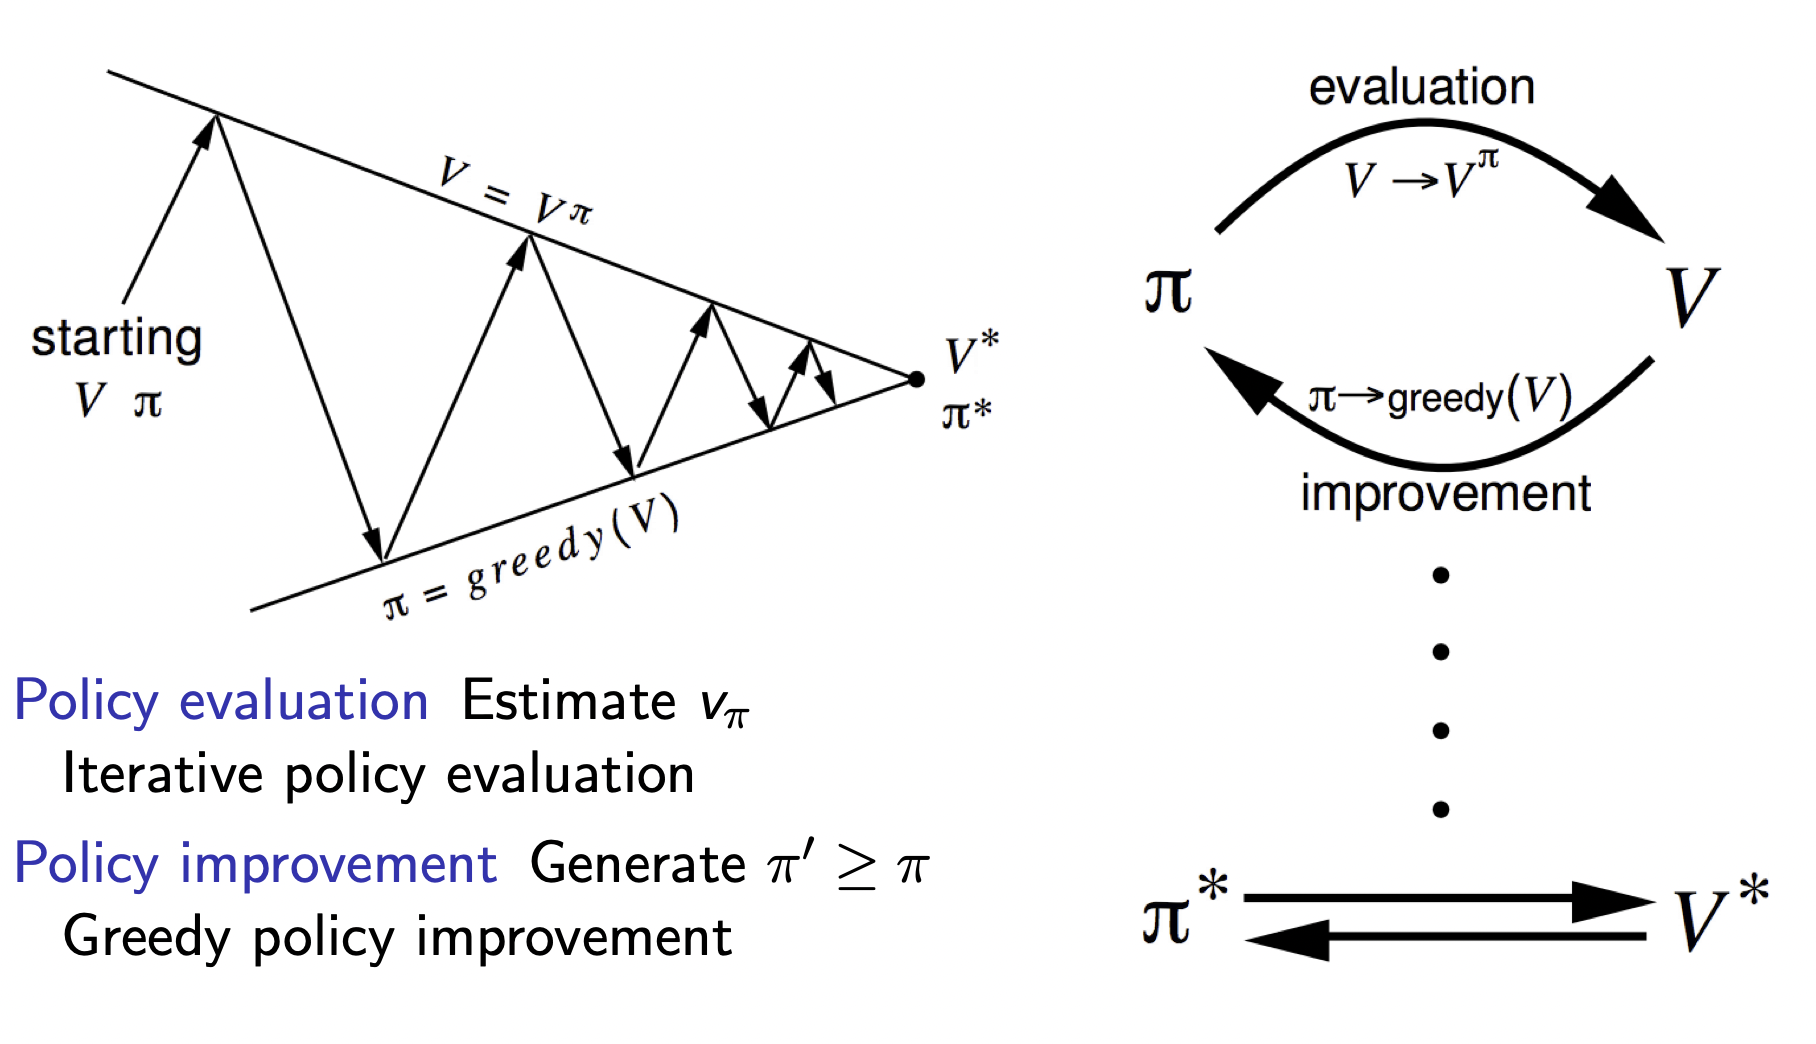
\includegraphics[scale=0.35]{pictures/eval_impr.png}

\subsubsection*{What does policy improvement mean?}
Consider a deterministic policy $a = \pi(s)$
\begin{itemize}
\item We can \textit{improve} the policy by acting greedily:  $\pi'(s) = \mathop{argmax}_{a \in \mathcal{A}} \; q_{\pi_{*}}(s,a)$
\item This will improve the value from any state s over one step: \\
$q_{\pi}(s, \pi'(s)) \;= \; \mathop{max}_{a \in \mathcal{A}} \; q_{\pi_{*}}(s,a) \; \geq \; q_{\pi_{*}}(s,a)\; + \; v_{\pi}$
\item Keep iterating over the coming time-steps
\item If improvement stops: \\
 $q_{\pi}(s, \pi'(s)) \;= \; \mathop{max}_{a \in \mathcal{A}} \; q_{\pi}(s,a) \; = \; q_{\pi}(s,a)\; = \; v_{\pi}$ \\
 $\qquad \rightarrow \qquad$ Bellman optimality equation is satisfied: $v_{\pi}(s)\;=\;\mathop{max}_{a \in \mathcal{A}} \; q_{\pi}(s,a)$
 \item Therefore: $v_{\pi} \; = \; v_{*}$ for all $s \in \mathcal{S} \qquad \rightarrow \qquad \pi$ is an optimal policy
\end{itemize}

\subsubsection*{Value iteration}
Any optimal policy can be subdivided into two components:
\begin{itemize}
\item An optimal first action $A_{*}$
\item Followed by an optimal policy from successor state $S'$
\end{itemize}
The policy is optimal, if from each state we might end up the policy is optimal from that state onwards.
If we know the solution to subproblems $v'_{*}(s)$, the solution $v_{*}(s)$ can be found iteratively by one-step lookahead:
\begin{equation}
v_{*}(s)\; \leftarrow \; \mathop{max}_{a \in \mathcal{A}}\: \left( \: \mathcal{R}_{s}^{a}\;+\;\gamma \sum_{s' \in \mathcal{S}} \mathcal{P}_{ss'}^{a}\:v_{*}(s') \: \right)
\end{equation}
The idea of value iteration is to apply these updates iteratively, thereby moving through the whole state-space. The intuition is that you begin with your final reward and work your way backwards.

Unlike policy iteration, there is no explicit policy. Intermediate value functions may not correspond to any policy.

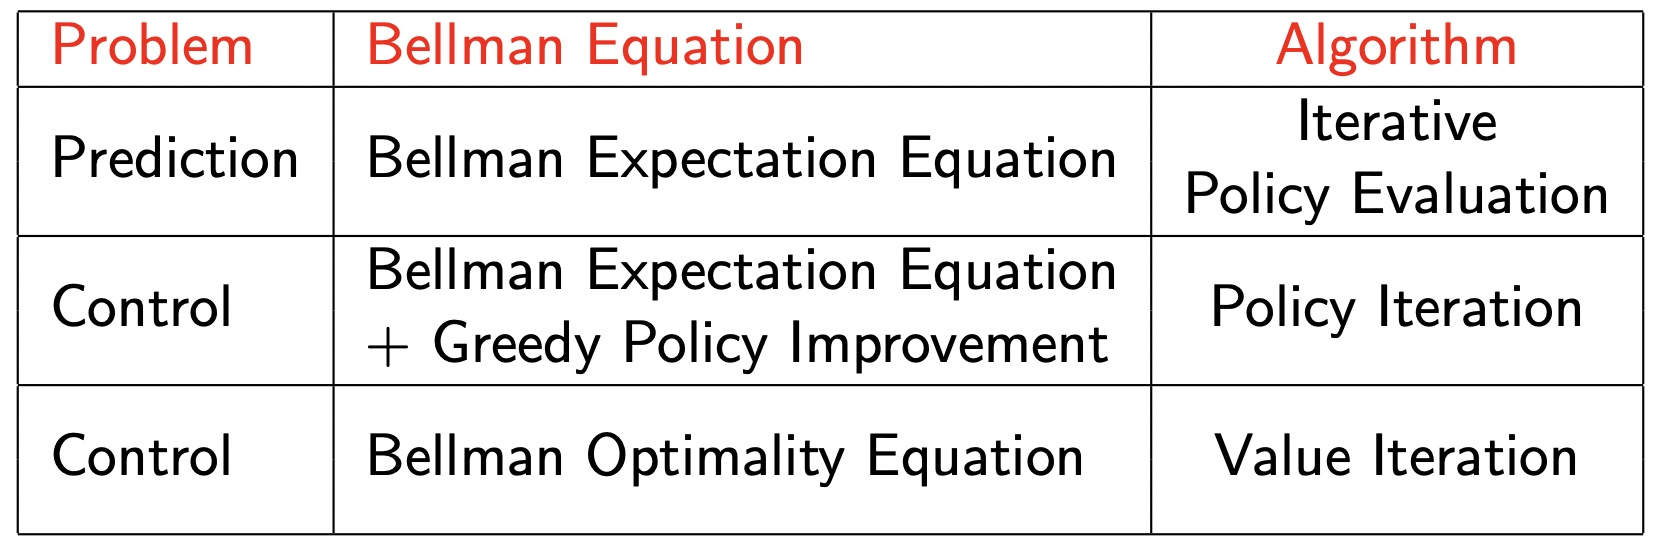
\includegraphics[scale=0.2]{pictures/synchronous_algorithms.jpg}

These algorithms are based on the state-value function $v_{\pi}(s)$ or $v_{*}(s)$. They have a complexity of $\mathcal{O}(mn^2)$ per iteration, for $m$ actions and $n$ states. The algorithms could also apply to $q_{\pi}(s)$ or $q_{*}(s)$, where the complexity would be $\mathcal{O}(m^{2}n^{2})$.

\subsection{Asynchronous dynamic programming}
It is not necessary to update every state at each sweep of the algorithm. In \textit{asynchronous} backups, the relationship of updating every state in each iteration is broken. This saves a lot of unnecessary work and as long as all states keep being selected at some time, the algorithm will still converge to the optimal solution.

\subsubsection*{In-place dynamic programming}
Synchronous value iteration stores two copies of the value function:
\begin{align}
v_{new}(s)\; \leftarrow \; \mathop{max}_{a \in \mathcal{A}}\: \left( \: \mathcal{R}_{s}^{a}\;+\;\gamma \sum_{s' \in \mathcal{S}} \mathcal{P}_{ss'}^{a}\:v_{old}(s') \: \right) \\ 
v_{old} \; \leftarrow \; v_{new}
\end{align}
In-place value iteration only stores one copy of value function by using the latest version of the value function available. That means if a state has been visited before, the algorithm uses the already calculated value instead of the old one. This tends to be more efficient, but the order of the states being swept is not relevant for the efficiency of the algorithm.

\subsubsection*{Prioritized sweeping}
By using the magnitude of the Bellman error to guide state selection, the states with the largest difference after an update have a higher priority. These will have the most effect in downstream computing. It is important though to update the Bellman error after each backup, which required knowledge of reverse-dynamics of a system for the predecessor states. The Bellman error is described as following:

\begin{equation}
\Big| \;  \mathop{max}_{a \in \mathcal{A}}\: \left( \: \mathcal{R}_{s}^{a}\;+\;\gamma \sum_{s' \in \mathcal{S}} \mathcal{P}_{ss'}^{a}\:v_{old}(s') \: \right) \; - \; v(s) \; \Big|
\end{equation}

\subsubsection*{Real-time Dynamic Programming}
The idea of \textit{Real-time programming} is to only update the states which are relevant to the agent. The experience of the agent is used to guide the the selection of states. After each time-step $S_{t}, A_{t}, R_{t+1}$, a backup of state $S_{t}$ is done.

\begin{equation}
v(S_{t})\; \leftarrow \; \mathop{max}_{a \in \mathcal{A}}\: \left( \: \mathcal{R}_{S_{t}}^{a}\;+\;\gamma \sum_{s' \in \mathcal{S}} \mathcal{P}_{S_{t}s'}^{a}\:v(s') \: \right) 
\end{equation}

\subsubsection*{Full-Width and Sample backups}
Dynamic programming uses \textit{full-width backups}, meaning that every state is backed up. For medium-sized problems consisting of a few millions of states, this is fine. But for large problems, dynamic programming suffer from the \textit{curse of dimensionality}, following from the exponential growth of the number of states with the number of state variables. 

This is where sample backups come into play. Instead of backing up the whole state-space (which can be already too expensive for one iteration), only certain samples are backed up. The advantages are:
\begin{itemize}
\item Model-free: No advance knowledge of MDP required
\item Breaks the curse of dimensionality through sampling
\item Cost of backup is constatnt, independant of $|n|=\mathcal{S}$ 
\end{itemize}
\newpage

\section{Lecture Four: Model-Free Prediction}
\subsection{Monte-Carlo Learning}
Monte-Carlo Learning methods learn directly from episodes of experience. It is therefore important that the MDP is applied to \textit{episodic} MDP, where the (complete) episodes do terminate. The value function is assumed to be the simplest possible, the mean return of the samples.

The goal is to learn the value function $v_{\pi}$ of a random policy $\pi$ by looking at some streams $S_{1}, A_{1}, R_{2}, \ldots, S_{k} \sim \pi$ of episode of experience and then evaluate the \textit{return} as the total discounted reward $\mathcal{G}_{t}$ form (\ref{eq:g_t}). Instead of using the \textit{expected} return of the value function, Monte-Carlo Learning uses the \textit{empirical mean} from the sampled episodes.

\subsubsection*{First-Visit Monte-Carlo policy evaluation}
\begin{itemize}
\item To evaluate the state $s$, the first time-step it is visited in an episode, an incremental counter is initialized: 
$N(s) \leftarrow N(s) + 1$
\item The total return is added up: $S(s) \leftarrow S(s) + G_{t}$
\item The value of the state is estimated by mean return: $V(s) = S(s) / N(s)$
\end{itemize}
By the law of large numbers, the value of the state $V(s)$ converges to the actual value $v_{\pi}$ of the state is visited many times so that the estimated mean consists of a large number of visits: $V(s) \rightarrow v_{\pi}$ as $N(s) \rightarrow \infty$

The \textbf{Every-Visit Monte-Carlo policy evaluation} works in a very similar fashion, just that the counter and return is incremented - as the name suggests - every time the episode visits a state.

\subsubsection*{Incremental Monte-Carlo}
The mean $\mu_{1}, \mu_{2}, \ldots$ of a sequence $x_{1}, x_{2}, \ldots$ can be computed incrementally:
\begin{equation}
\begin{aligned}
\mu_{k}\; &=\;\frac{1}{k}\:\sum_{j=1}^{k}\:x_{j}\\
&=\;\frac{1}{k}\:\big( x_{k} \:+\: \sum_{j=1}^{k-1}\:x_{j}\: \big) \\
&=\;\frac{1}{k}\:(\:x_{k} \: + \: (k-1)\:\mu_{k-1} \: )\\
&=\; \mu_{k-1} \: + \: \frac{1}{k}\:(\:x_{k} \: - \:\mu_{k-1} \: )
\end{aligned}
\label{eq:incr_mean}
\end{equation}
The difference $x_{k} - \mu_{k-1}$ basically defines the error term, where $\mu_{k-1}$ represents the expected value and $x_{k}$ the actual value. In the process of (\ref{eq:incr_mean}), the value of the mean will then get an update slightly into the direction of the error term.

This can be applied to the Monte-Carlo Learning. The value $V(s)$ of a state $s$ will be updated incrementally after an episode $S_{1}, A_{1}, R_{2}, \ldots, S_{t}$:
\begin{itemize}
\item For each state $S_{t}$ with return $G_{t}$: \\
$N(s) \leftarrow N(s) + 1$ \\
$V(S_{t}) \leftarrow V(S_{t}) + \frac{1}{N(s)} (G_{t} - V(S_{t}))$
\item In non-stationary problems, it can be useful to track a running mean, e.g. forget old episodes \\
$V(S_{t}) \leftarrow V(S_{t}) + \alpha (G_{t} - V(S_{t}))$
\end{itemize}

\subsection{Temporal-Difference Learning}
Like with Monte-Carlo Learning, Temporal-Difference Learning learns from episodes of experience and needs no knowledge of the MDP transitions or rewards, they are both \textit{model-free}. In contrast to Monte Carlo Learning however, Temporal-Difference Learning also learns from incomplete episodes, they don't have to terminate. By taking partial episodes and estimating the remaining return, it can learn from incomplete episodes. It iteratively updates the guesses of the return while going thorugh an episode. This is called \textit{bootstrapping}.

\subsubsection*{The simplest Temporal-Difference Learning algorithm: TD(0)}
\begin{itemize}
\item The value of $V_{s}$ is updated towards the \textit{estimated} return: $R_{t+1}+\gamma V(S_{t+1})$
\begin{align*}
V(S_{t}) \leftarrow V(S_{t}) + \alpha (R_{t+1}+\gamma V(S_{t+1}) - V(S_{t}))
\end{align*}
\item $R_{t+1}+\gamma V(S_{t+1})$     is called the TD target (the estimated return)
\item $\delta_{t} = (R_{t+1}+\gamma V(S_{t+1}) - V(S_{t}))$     is called the TD error
\end{itemize}

\begin{figure}
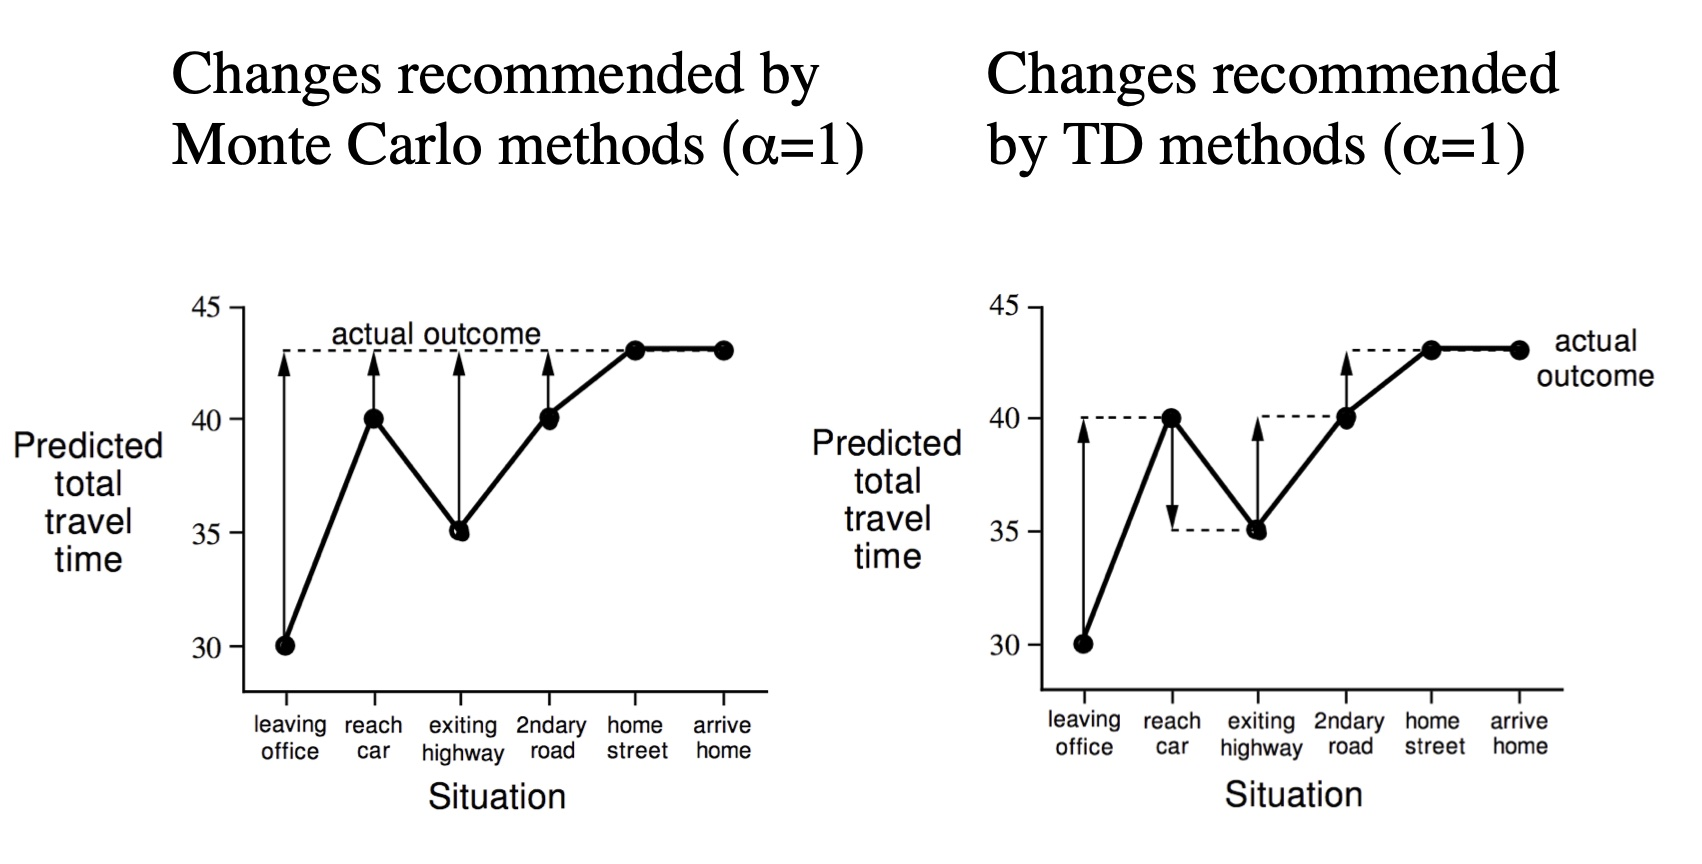
\includegraphics[scale=0.2]{pictures/mc_td.jpg}
\caption{The difference between Monte-Carlo and Temporal-Difference Learning.}
\label{img:mc_td}
\end{figure}

As seen in caption \ref{img:mc_td}, the predicted total travel time gets updated after every state in TD Learning, while in MC learning all the values of the states will be updated after the episode.

\subsubsection*{Advantages and Disadvantages of Temporal-Difference vs. Monte-Carlo Learning}

\begin{itemize}
\item TD can learn before knowing the final outcome
\begin{itemize}
\item TD can learn online after every step
\item MC must wait until the end of an episode before return is known
\end{itemize}
\item TD can learn without the final outcome
\begin{itemize}
\item TD can learn from incomplete sequences
\item MC can only learn from complete sequences
\item TD works in continuing environments
\item MC only works for episodic (terminating) environments
\end{itemize}
\item Certainty equivalence:
\begin{itemize}
\item MC converges to solution with minimal mean-squared error \\ $ \rightarrow$ Best fit to the observed returns
\item TD converges to solution of max likelihood Markov model \\ $ \rightarrow$ Solution to the MDP that best fits the data
\end{itemize}
\item TD exploits Markov property by using it, therefore is more efficient in a Markov environment. MC ignores the Markov property, therefore does not exploit it.
\end{itemize}

\subsubsection*{Bias / Variance Trade-Off}
\begin{itemize}
\item The return $G_{t}$ and the true TD target $R_{t+1}+\gamma v_{\pi}(S_{t+1})$ are both \textit{unbiased} estimates of $v_{\pi}(S_{t})$. 
\item The actual TD target $R_{t+1}+\gamma V(S_{t+1})$ is a \textit{biased} estimate of $v_{\pi}(S_{t})$. It is much lower variance than the return:
\begin{itemize}
\item Return depends on \textit{many} random actions, transitions and rewards.
\item TD target depends on \textit{one} random action, transition and reward.
\end{itemize}
\item MC has high variance, zero bias
\begin{itemize}
\item Good convergence properties, even with function approximation
\item Not very sensitive to initial value
\item Very simple to understand and use.
\end{itemize}
\item TD has low variance, some bias
\begin{itemize}
\item Usually more efficient than MC
\item TD(0) converges to $v_{\pi}(s)$ - but not always with function approximation
\item More sensitive to initial value
\end{itemize}
\end{itemize}


\begin{center}
\begin{minipage}[t]{0.45\textwidth}
\textbf{Monte-Carlo Backup:}
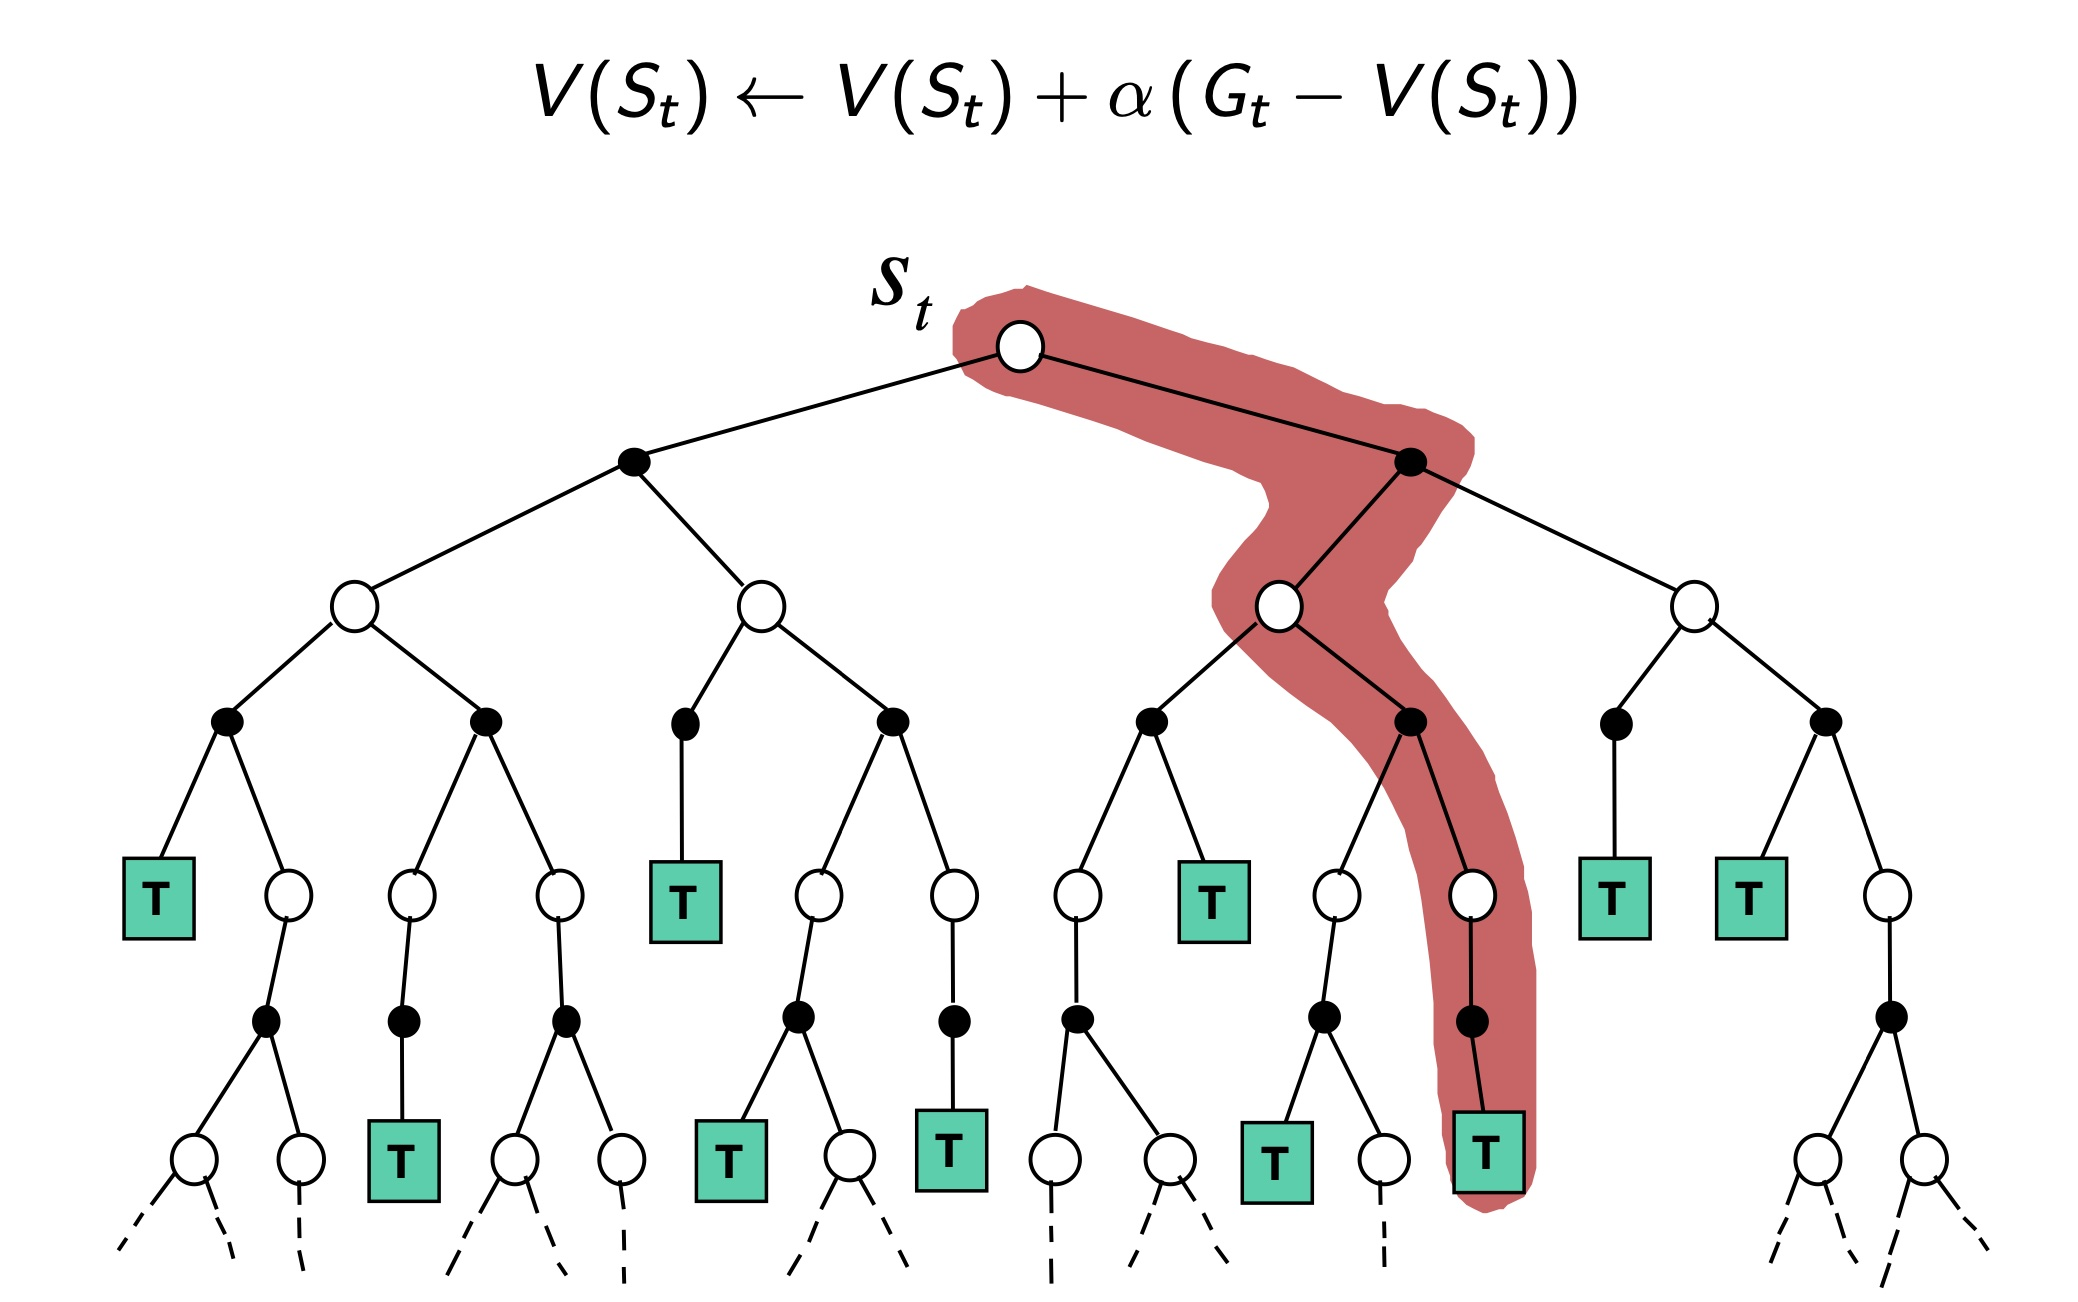
\includegraphics[width=\textwidth]{pictures/mc_backup.jpg}
\end{minipage} \hfill
\begin{minipage}[t]{0.45\textwidth}
\textbf{Temporal-Difference Backup:}
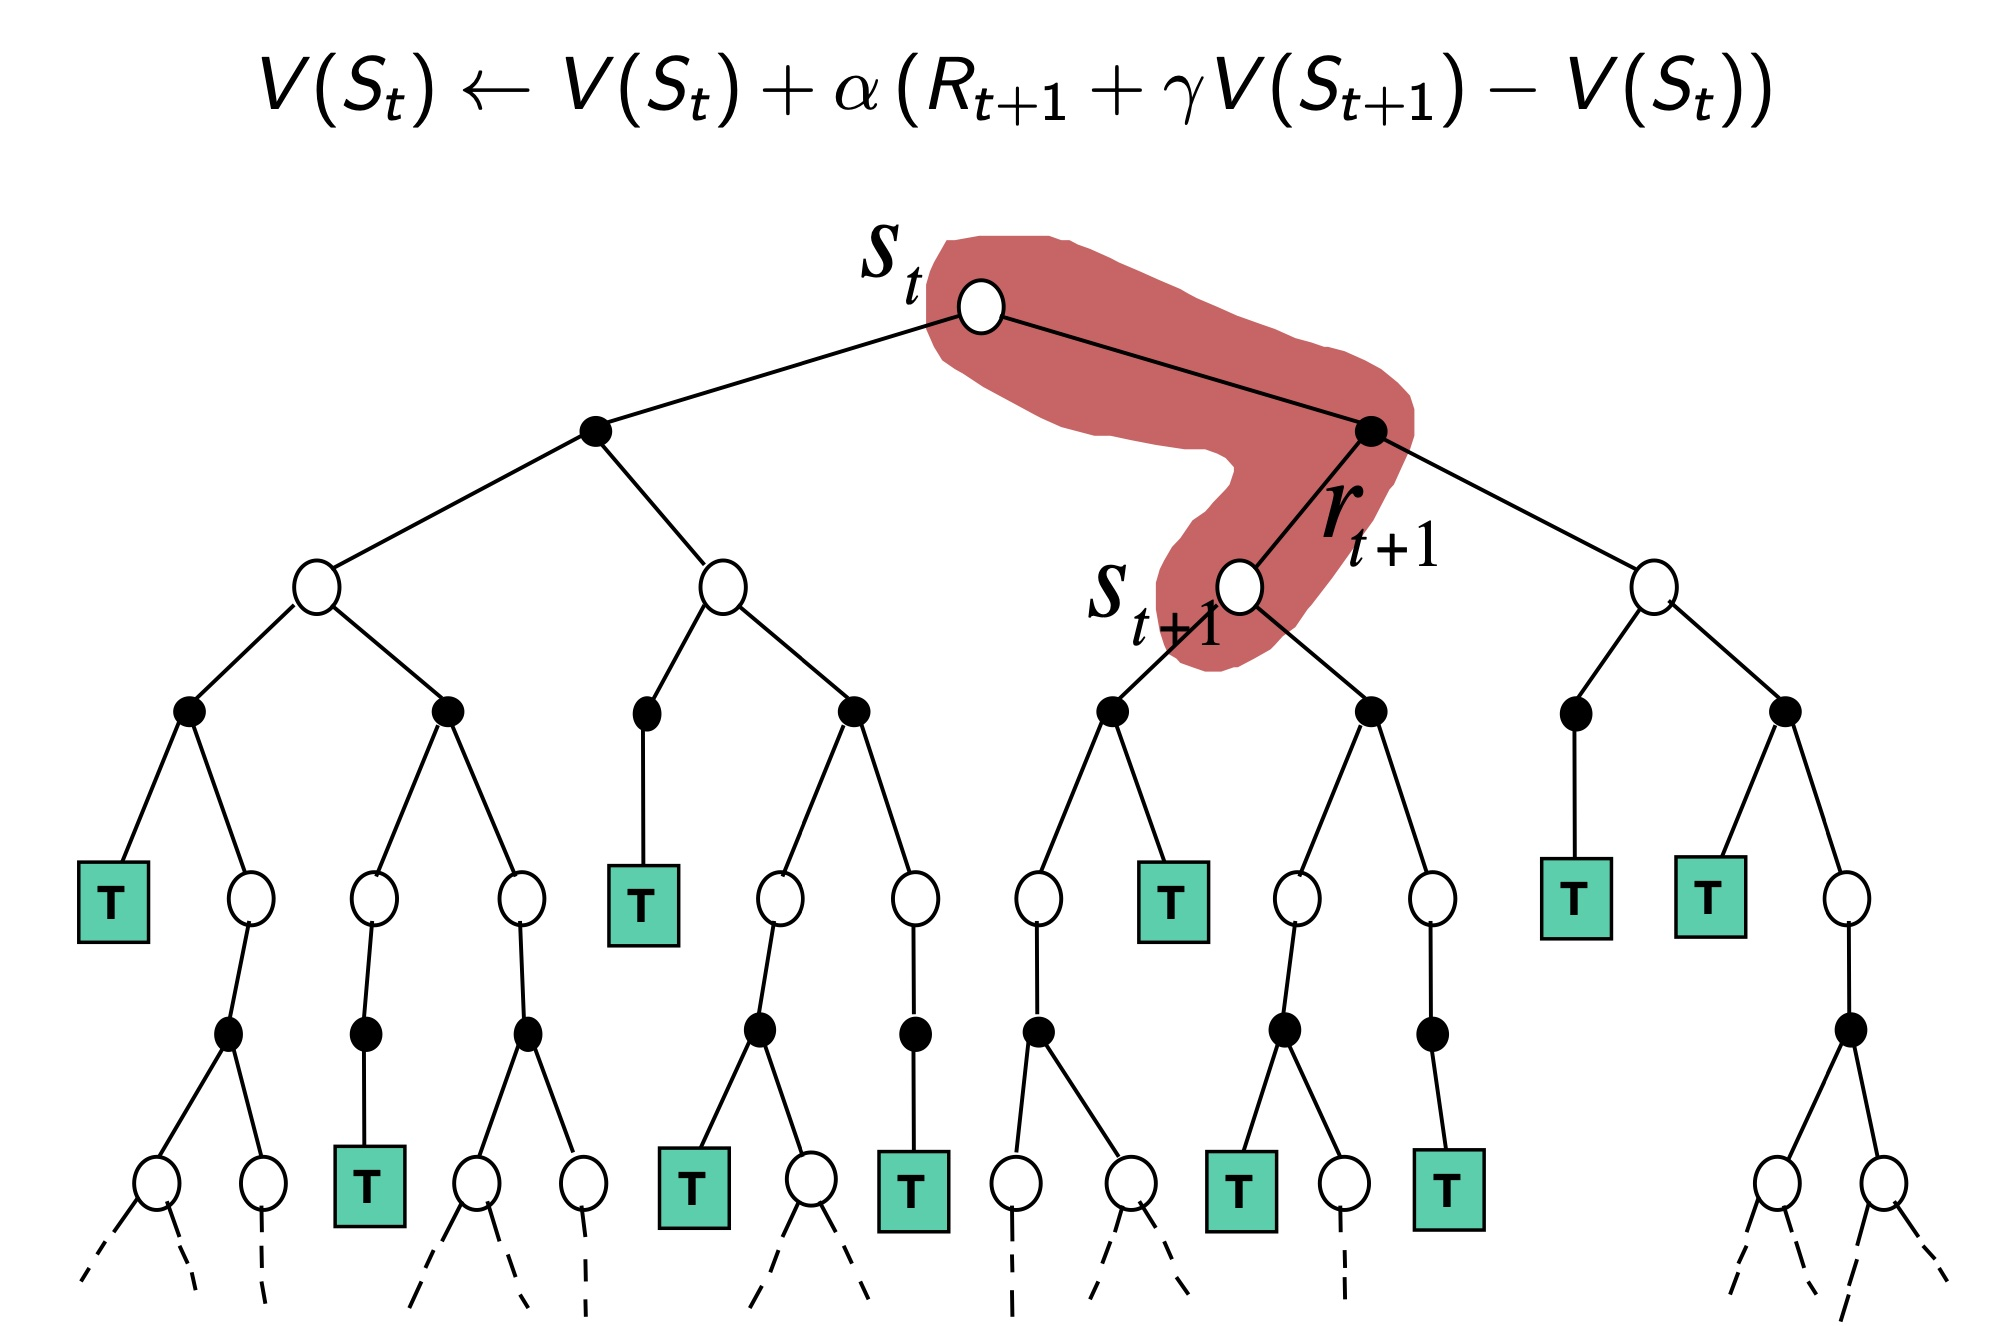
\includegraphics[width=\textwidth]{pictures/td_backup.jpg}
\end{minipage}
\newline \newline \newline
\begin{minipage}[t]{0.45\textwidth}
\textbf{Dynamic Programming Backup:}
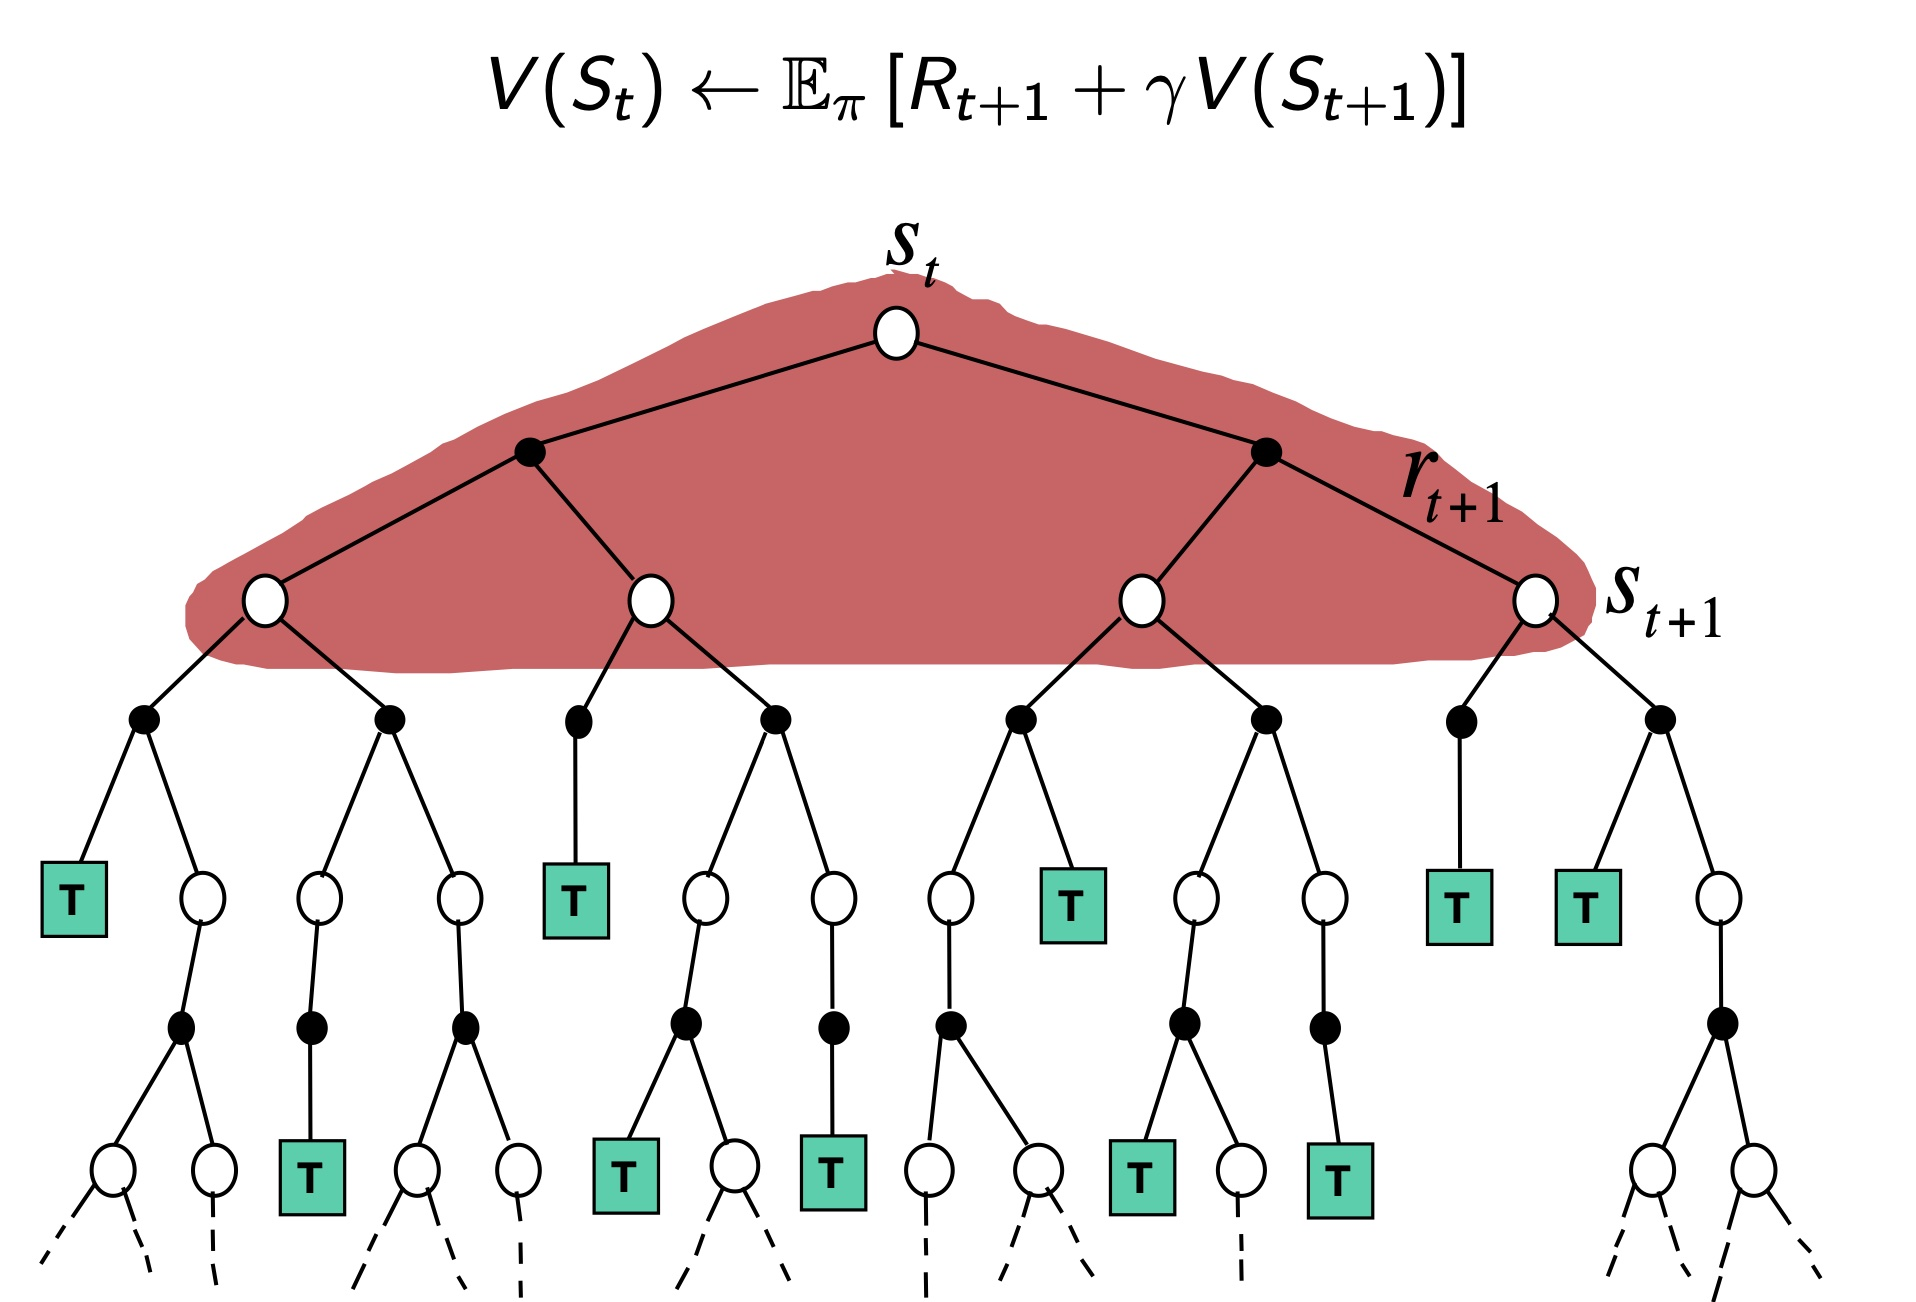
\includegraphics[width=\textwidth]{pictures/dp_backup.jpg}

Note: The \textit{'Exhaustive search'} would consider every branch as in Dynamic Programming, but then follow its leafs until the end like Monte-Carlo instead of taking an estimate.
\end{minipage} \hfill
\begin{minipage}[t]{0.4\textwidth}
\begin{itemize}
\item \textbf{Bootstrapping:} \\ update involves an estimate
\begin{itemize}
\item MC does not bootstrap
\item TD and DP do
\end{itemize}
\item \textbf{Samling:} \\ update samples an expectation
\begin{itemize}
\item MC and TD sample
\item DP does not sample
\end{itemize}
\end{itemize}
\end{minipage}
\end{center}
\newpage
\begin{figure}
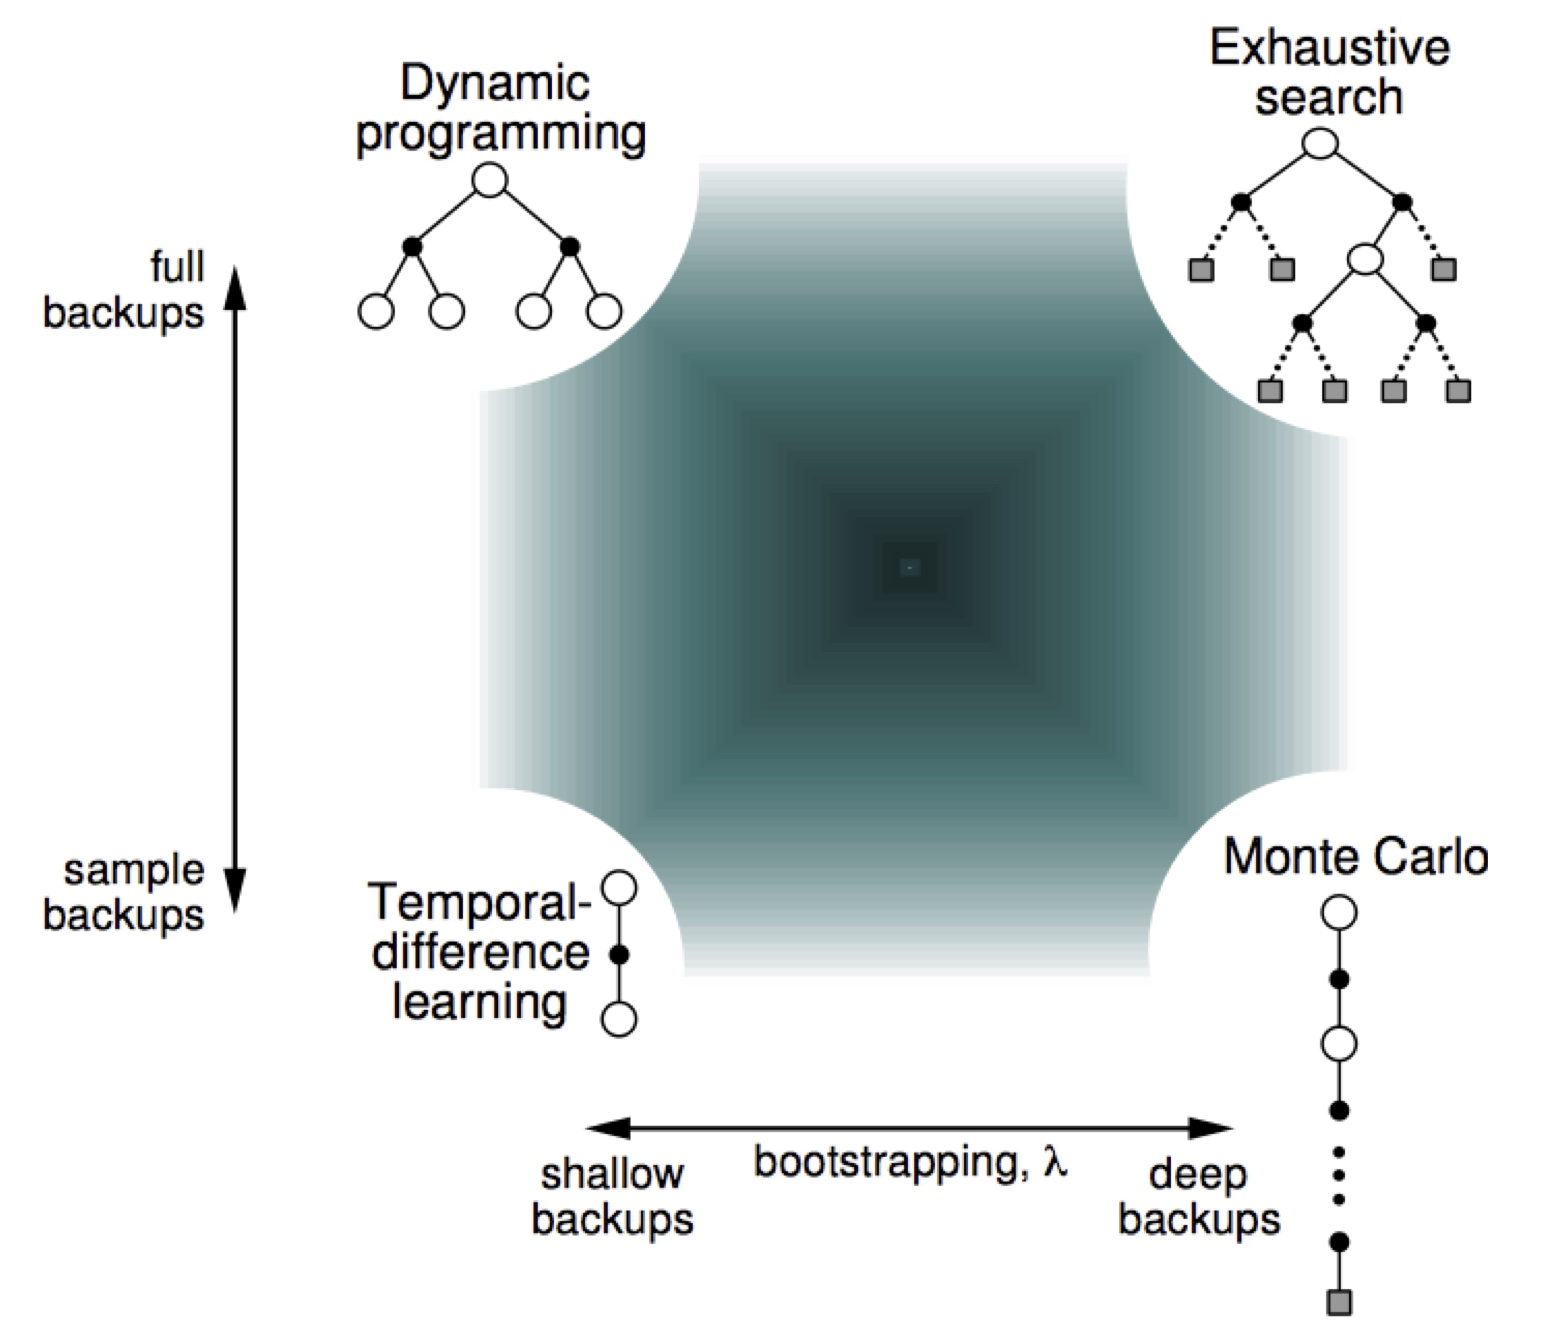
\includegraphics[width=0.7\textwidth]{pictures/unified_view.jpg}
\caption{Unified view of Reinforcement Learning}
\end{figure}

\subsection{TD($\lambda$)}
\subsubsection*{n-step Prediction}

\begin{figure}[h!]
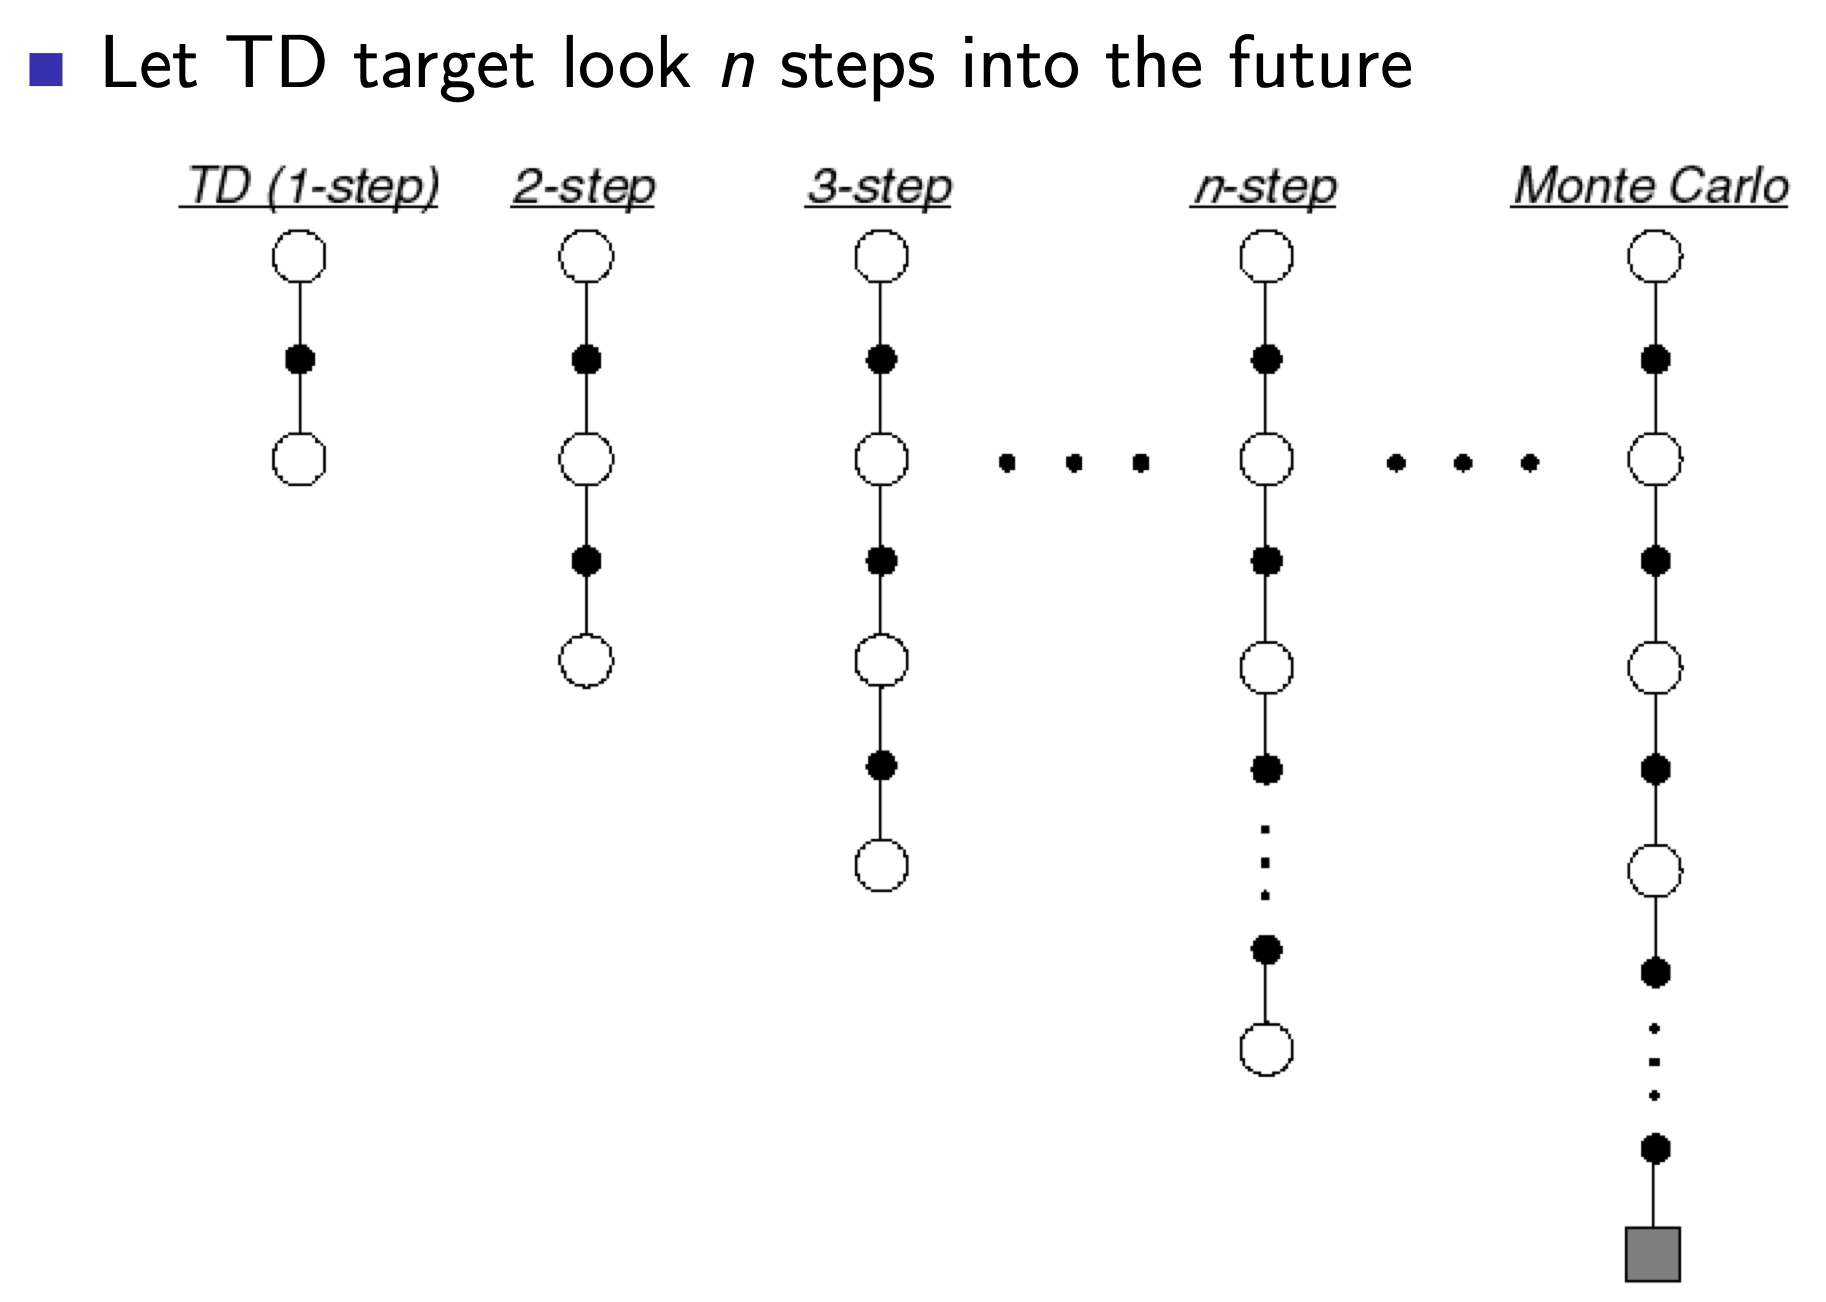
\includegraphics[width=0.7\textwidth]{pictures/n_step_pred.jpg}
\end{figure}
\subsubsection*{n-step Return}
\begin{align*}
n=1 \quad & (TD) \quad &G_{t}^{(1)} \; &= \; R_{t+1} \:  \gamma V(S_{t+1}) \\
n=2 \quad & \quad \quad &G_{t}^{(2)} \; &= \; R_{t+1} \:  \gamma R_{t+2} \: + \: \gamma^{2} V(S_{t+2}) \\
\vdots \quad &\quad \quad &\vdots & \\
n=\infty \quad & (MC) \quad &G_{t}^{(\infty)} \; &= \; R_{t+1} \: + \:  \gamma R_{t+2} \: + \: \gamma^{T-1} R_{T}
\end{align*}

Define the \textit{n}-step return for the estimator:
\begin{equation}
G_{t}^{(n)} \; = \; R_{t+1} \: + \: \gamma R_{t+2} \: + \ldots \: + \: \gamma^{n-1} R_{t+n} \: + \: \gamma^{n} V(S_{t+n}) 
\end{equation}

\textit{n}-step Temporal-Difference Learning:
\begin{equation}
V(S_{t}) \leftarrow V(S_{t}) + \alpha (G_{t}^{(n)} - V(S_{t})
\end{equation}

\subsubsection*{Forward-view of TD($\lambda$)}
\begin{minipage}{0.5\textwidth}
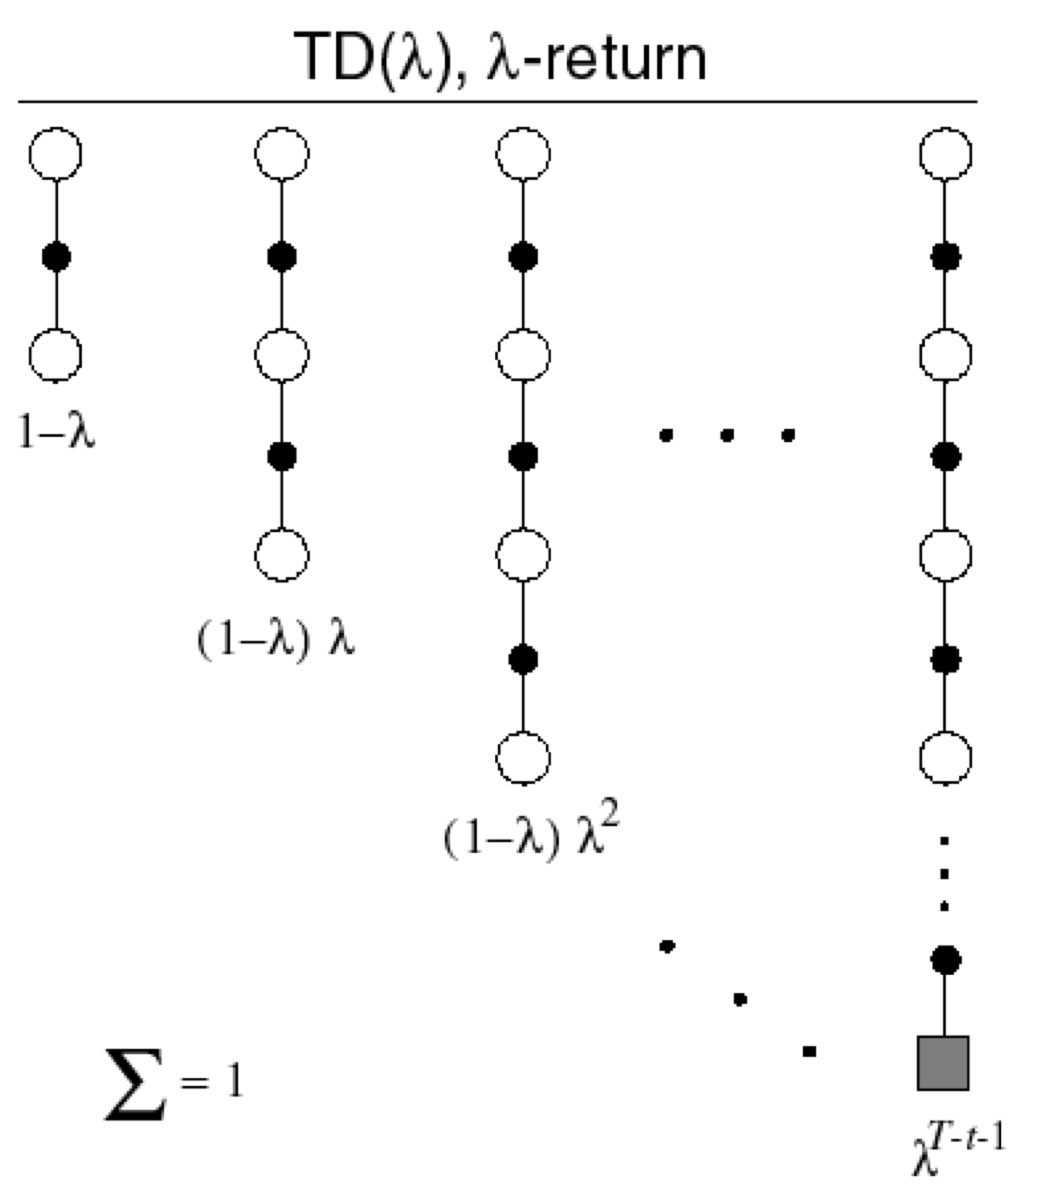
\includegraphics[width=\textwidth]{pictures/lambda_return.jpg}
\end{minipage} \hfill
\begin{minipage}{0.5\textwidth}
The $\lambda$-return $G_{t}^{(\lambda)}$ combines all $n$-step returns $G_{t}^{(n)}$  \\ \\
Using weight $(1-\lambda)\lambda^{n-1}$:
\begin{equation}
G_{t}^{\lambda}\;=\; (1-\lambda)\:\sum_{n=1}^{\infty} \lambda^{n-1} \: G_{t}^{(n)}
\label{eq:fw-lambda} \end{equation}
By using this to update the value function, we get the Forward-view TD($\lambda$)
\begin{equation}
V(S_{t}) \leftarrow V(S_{t}) + \alpha (G_{t}^{\lambda} - V(S_{t}))
\end{equation}
\end{minipage}


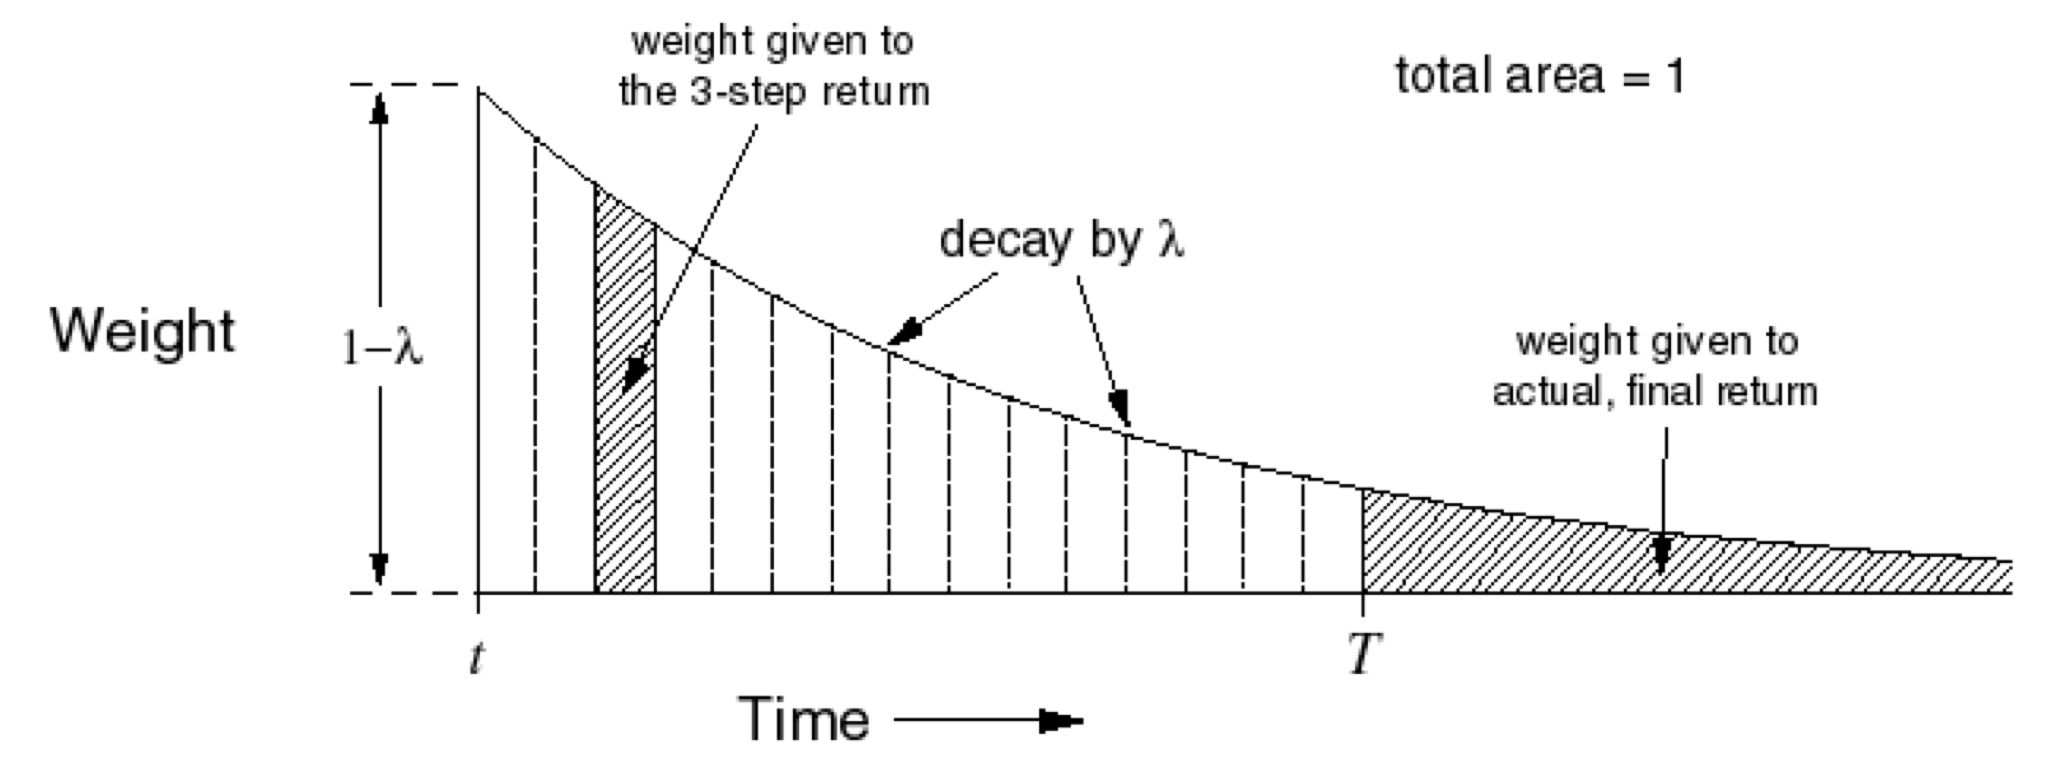
\includegraphics[width=0.9\textwidth]{pictures/tdl_weight.jpg}

The Forward-view looks into the future to compute $G_{t}^{(\lambda)}$. Like Monte-Carlo Learning, it can only be computed from complete episodes.
\newpage
\subsubsection*{Backward-view of TD($\lambda$)}

\begin{center}

\textit{The Forward-view provides theory, the Backward-view provides mechanism}
\end{center}
It updates online, every step, from incomplete sequences. \newline

\begin{itemize}
\item \textbf{Frequency heuristic:} Assign credit to most frequent states
\item \textbf{Recency heuristic:} Assign credit to most recent states
\end{itemize}
$\qquad \rightarrow \quad$ \textit{Eligibility traces} combine both heuristics!

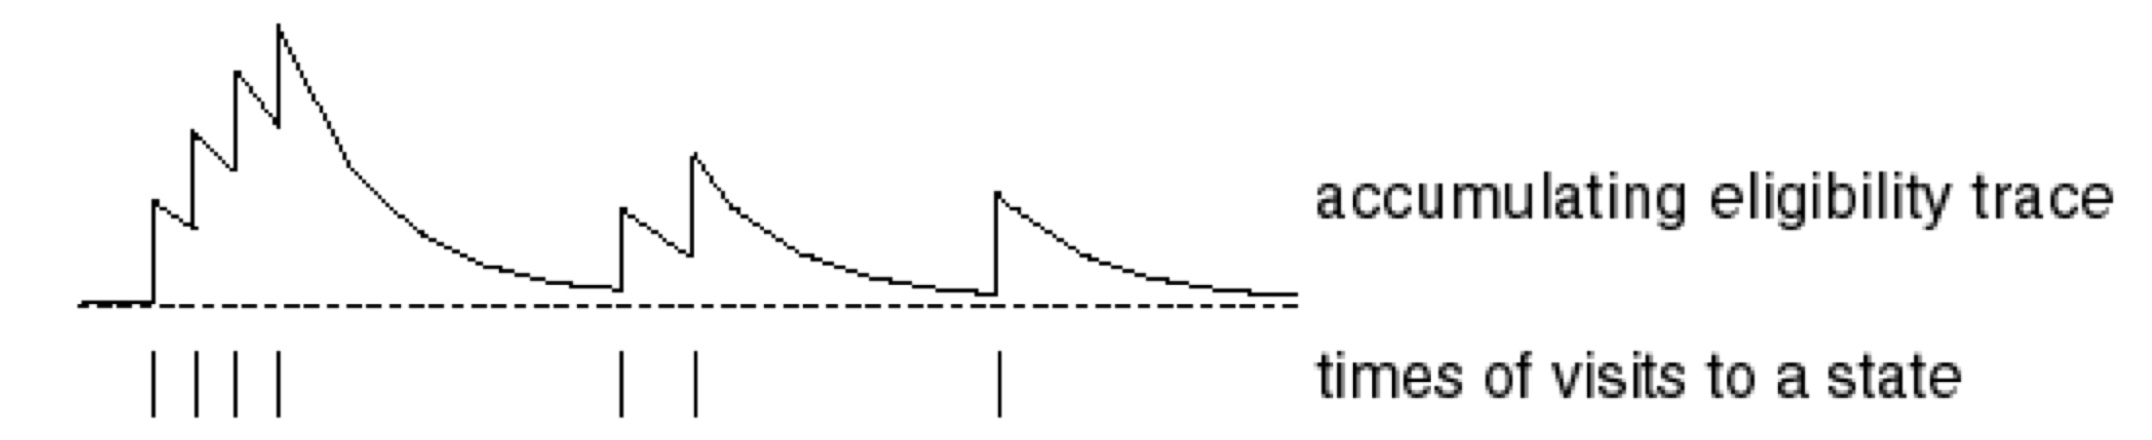
\includegraphics[width=0.75\textwidth]{pictures/eli_trace.jpg}

\begin{align*}
E_{0}(s) \; &= \; 0 \\
E_{t}(s) \; &= \gamma \lambda E_{t-1}(s)\: + \: \mathbf{1}(S_{t} =s)
\end{align*}

Backward-view TD($\lambda$)-Algorithm:
\begin{itemize}
\item Keep an eligibility trace for every state $s$
\item Update value $V(s)$ for every state $s$
\item In proportion to TD-error $\delta_{t}$ and eligibility trace $E_{t}(s)$
\begin{align}
\delta_{t} \; &= \; R_{t+1} \: + \: \gamma V(S_{t+1}) - V(S_{t}) \\
V(s) \; &\leftarrow \; V(s) \: + \: \alpha \delta_{t} E_{t}(s)
\end{align}
\end{itemize}

\subsubsection*{Relationship between Forward and Backward TD($\lambda$)}

The sum of the offline\footnote{Even for online updating it is now possible to achieve equivalence for forward and backward view TD($\lambda$) - see } updates is the same identical for forward-view and backward-view TD($\lambda$)

\begin{equation}
\sum_{t=1}^{T}\:\alpha \delta_{t} E_{t}(s)\;=\;\sum_{t=1}^{T}\alpha (G_{t}^{\lambda} - V(S_{t})) \: \mathbf{1}(S_{t} =s)
\end{equation}
\begin{center}
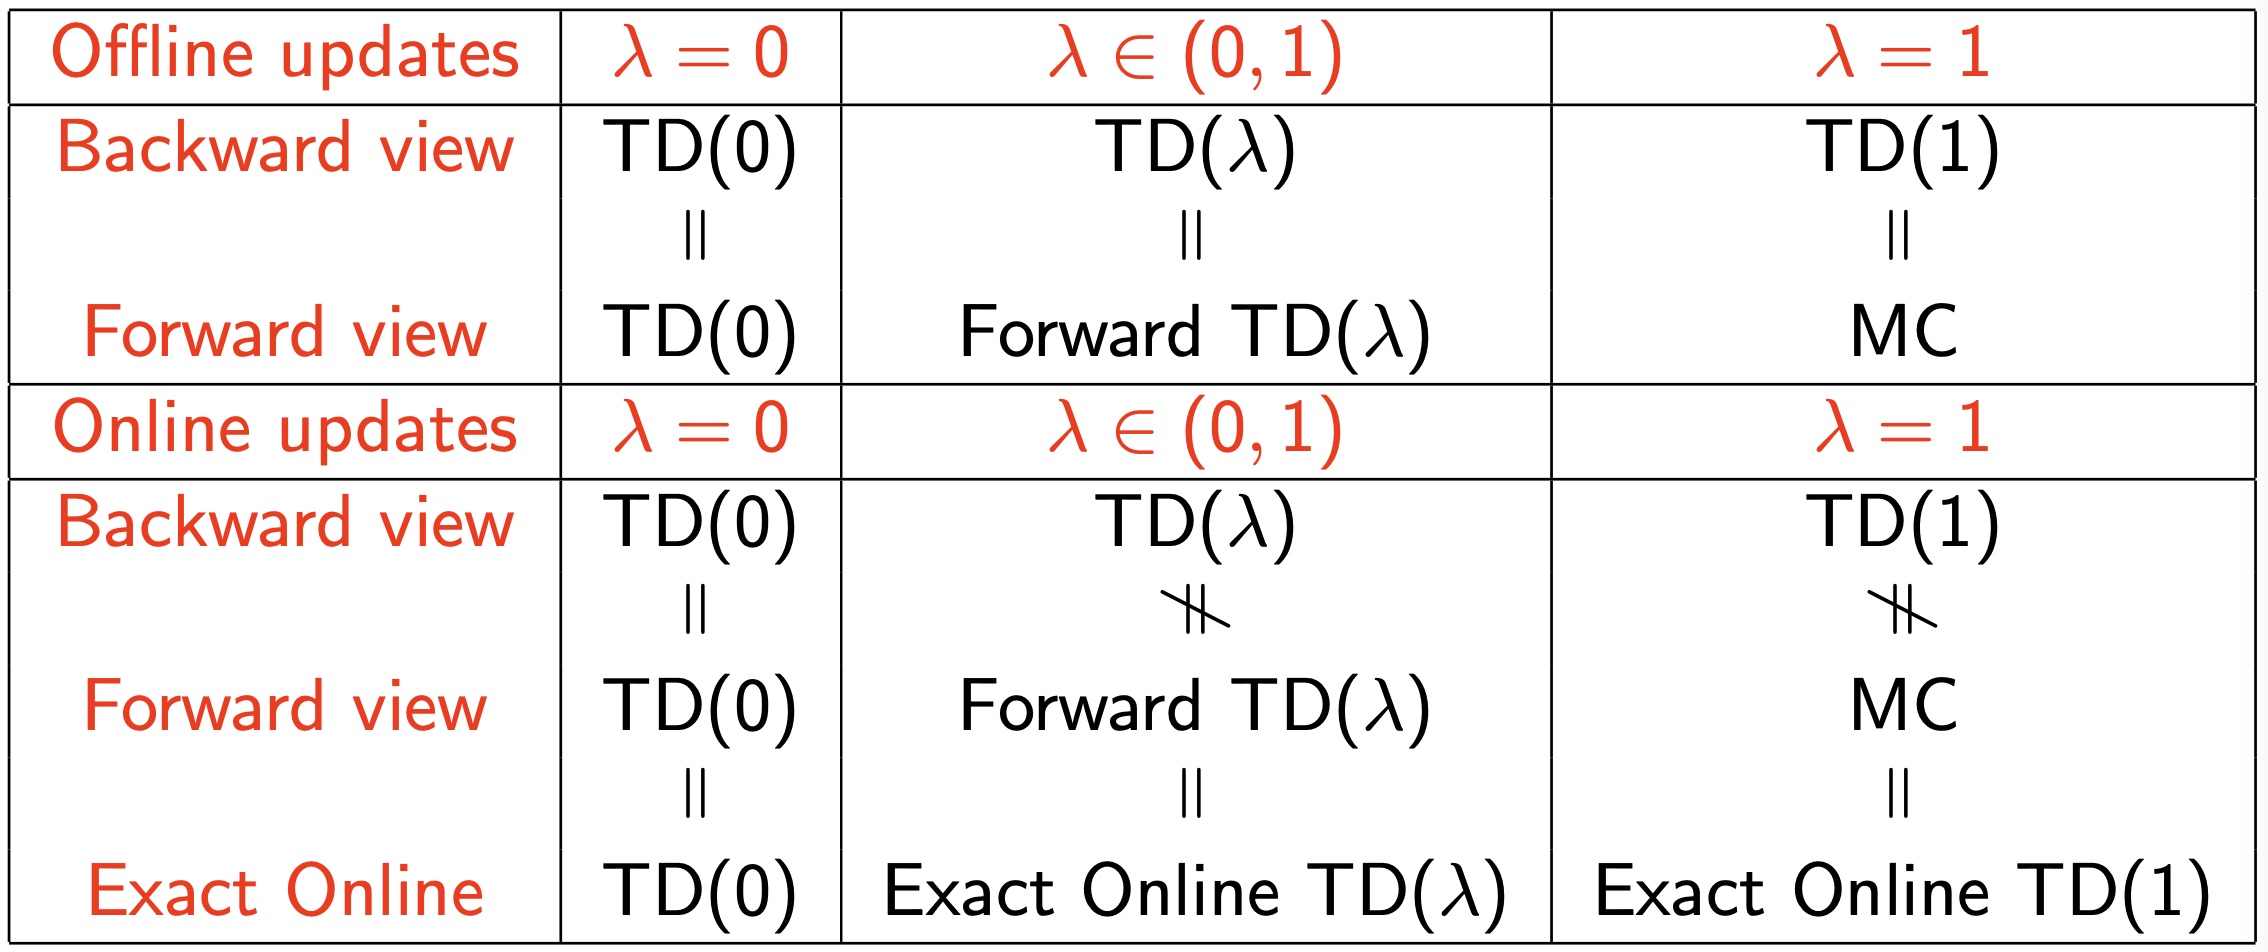
\includegraphics[width=0.7\textwidth]{pictures/overview_tdl.jpg}
\end{center}

\section{Model-Free Control}
\begin{center}
\textbf{Model-free prediction:} \textit{Estimate} the value function of an \textit{unknown} MDP
\textbf{Model-free control:} \textit{Optimise} the value function of an \textit{unknown} MDP
\end{center}


Model-free control can solve problems whether either the MDP model is unknown, but experience can be sampled or where the MDP model is known but too big to use - except by samples (e.g. when the underlying real-world dynamics are very complicated).

\subsection{On and Off-policy learning}
\subsubsection*{On-policy learning:}
\begin{itemize}
\item "Learn on the job"
\item "Learn about policy $\pi$ from experience sampled from $\pi$
\end{itemize}

\subsubsection*{Off-policy learning:}
\begin{itemize}
\item "Look over someone's shoulder"
\item "Learn about policy $\pi$ from experience sampled from $\mu$
\end{itemize}

\subsubsection*{Model-Free Policy iteration using action-value function}

Greedy policy improvement over the state value function $V(s)$ requires a model of the MDP:
\begin{equation}
\pi'(s) \; = \; \mathop{argmax}_{a \in \mathcal{A}} \mathcal{R}_{s}^{a} \: + \: \mathcal{P}_{ss;}^{a} V(s')
\end{equation}
...whereas greedy policy improvement over the action value function $Q(s,a)$ is model-free
\begin{equation}
\pi'(s) \; = \; \mathop{argmax}_{a \in \mathcal{A}} Q(s,a)
\end{equation}

\subsection{$\epsilon$-Greedy Exploration}
This is them simplest idea for ensuring continual exploration.
\begin{itemize}
\item All \textit{m} actions are tried with non-zero probability
\item With probability 1-$\epsilon$ choose the greedy action
\item With probability $\epsilon$ choose an action at random 
\end{itemize}

\begin{equation}
\pi(a|s)\; = \; \Big\{ \; \begin{matrix} \epsilon/m+1-\epsilon \qquad & $if$ \quad a* = \mathop{argmax}_{a \in \mathcal{A}} Q(s, a) \\
\epsilon / m & $otherwise$ \\\end{matrix} 
\end{equation}

\newpage
\textbf{GLIE:} Greedy in the Limit with Infinite Exploration
\begin{itemize}
\item All state-action pairs are explored infinitely many times: \\
$\mathop{lim}_{k \rightarrow \infty} N_{k} (s, a) = \infty$
\item The policy converges on a greedy policy \\
$\mathop{lim}_{k \rightarrow \infty} \pi_{k}(a|s) = \mathbf{1}(a = \mathop{argmax}_{a' \in \mathcal{A}}\: Q_{k}(s, a')) \\ \\
\rightarrow \quad$ for example, $\epsilon$-greedy is GLIE if $\epsilon$ reduces to zero at $\epsilon_{k} = \frac{1}{k}$
\end{itemize}

\subsubsection*{GLIE Monte-Carlo Control}

\begin{itemize}
\item Sample \textit{k}-th epsidoe using $\pi: {S_{1}, A_{1}, R_{2}, \ldots, S_{T} } \sim \pi$
\item For each state $S_{T}$ and action $A_{T}$ in the episode,
\begin{align*}
N(S_{t}, A_{t}) \; &\leftarrow \; N(S_{t}, A_{t}) \: + \: 1 \\
Q(S_{t}, A_{t}) \; &\leftarrow \; Q(S_{t}, A_{t})) \: + \: \frac{1}{N(S_{t}, A_{t})} (G_{t} - Q(S_{t}, A_{t}))
\end{align*}
\item Improve policy based on new action-value function
\begin{align*}
 \epsilon \; &\leftarrow \; 1/l \\ \pi \; &\leftarrow \;  \epsilon - greedy(Q)	
\end{align*}
\end{itemize}

\subsection{TD($\lambda$) Control}

\subsubsection*{MC vs. TD control}

Temporal difference (TD) Learning has several advantages over Monte-Carlo (MC):
\begin{itemize}
\item Lower variance
\item online
\item Incomplete sequences
\end{itemize}
Natural idea: use TD instead of MC in our control loop
\begin{itemize}
\item Apply TD to Q(S, A)
\item Use $\epsilon$-greedy policy improvement
\item Update every time step
\end{itemize}
\newpage

\subsubsection*{Updating Action-Value Functions with \textit{Sarsa}}

\begin{figure}[h!]
\begin{center}
\includegraphics[width=0.25\textwidth]{pictures/sarsa.jpg}
\end{center}
\end{figure}
\begin{equation} \small
Q^{new}\:(s_{t}, a_{t})  = \underbrace{Q(s_{t}, a_{t})}_{\text{current value}}  + \underbrace{\alpha}_{\text{learning rate}} \cdot 
\overbrace{\Bigl( \underbrace{\underbrace{r_{t}}_{\text{reward}} + \underbrace{\gamma}_{\text{discount factor}} \cdot \underbrace{\mathop{max}_{a \in \mathcal{A}} Q(s_{t}, a_{t+1})}_{\text{estimate of optimal future value}}}_{\text{new value (temporal difference target)}} - \underbrace{Q(s_{t}, a_{t})}_{\text{current value}} \Bigr) }^{\text{temporal difference}}
\end{equation}
The \textit{Sarsa}-algorithm for on-policy learning would be the following:
\begin{figure}[h!]
\begin{center}
\includegraphics[width=0.8\textwidth]{pictures/sarsa_alg.jpg}
\end{center}
\end{figure}

\textbf{$\rightarrow$ \textit{n}-Step Sarsa}

\begin{align*}
n=1 \quad & (Sarsa) \quad &q_{t}^{(1)} \; &= \; R_{t+1} \:  \gamma Q(S_{t+1}) \\
n=2 \quad & \quad \quad &q_{t}^{(2)} \; &= \; R_{t+1} \:  \gamma R_{t+2} \: + \: \gamma^{2} Q(S_{t+2}) \\
\vdots \quad &\quad \quad &\vdots & \\
n=\infty \quad & (MC) \quad &q_{t}^{(\infty)} \; &= \; R_{t+1} \: + \:  \gamma R_{t+2} \: + \: \gamma^{T-1} R_{T}
\end{align*}

Define the \textit{n}-step Q-return:
\begin{equation}
q_{t}^{(n)} \; = \; R_{t+1} \: + \: \gamma R_{t+2} \: + \ldots \: + \: \gamma^{n-1} R_{t+n} \: + \: \gamma^{n} Q(S_{t+n}) 
\end{equation}

\textit{n}-step Sarsa updates Q(s, a) towards the \textit{n}-step Q-return
\begin{equation}
Q(S_{t}, A_{t}) \leftarrow Q(S_{t}, A_{t}) + \alpha \bigl( q_{t}^{(n)} - Q(S_{t}, A_{t}) \bigr)
\end{equation}

By following the same logic as for TD($\lambda$) in (\ref{eq:fw-lambda}) and using weight $(1-\lambda) \lambda^{n-1}$
\begin{equation}
q^{\lambda}_{t} = (1-\lambda) \sum_{n=1}^{\infty} \lambda^{n-1}q^{(n)}_{t}
\end{equation}

... we get the \textbf{Forward-view Sarsa($\lambda$)}
\begin{equation}
Q(S_{t}, A_{t}) \leftarrow Q(S_{t}, A_{t}) + \alpha \bigl( q_{t}^{(\lambda)} - Q(S_{t}, A_{t}) \bigr)
\end{equation}

Just like TD($\lambda$), we use \textit{eligibility traces} in an online algorithm for \textbf{Backward-View Sarsa($\lambda$)}. Is this case, Sarsa($\lambda$) has one eligibility trace for each state-action pair:

\begin{align}
E_{0} (s, a) \; &= \; 0 \\
E_{t} (s, a) \; &= \; \gamma \lambda E_{t-1}(s, a) + \underbrace{\mathbf{1}(S_{t} = s, A_{t}}_{\text{increment by 1 each time the state-action pair is visited}}
\end{align}

\textit{Q(s, a)} is updated for every state \textit{s} and \textit{a} in proportion to TD-error $\delta_{t}$ and eligibility trace $E_{t}(s, a)$:
\begin{align}
\delta_{t} \; &= \; R_{t+1} + \gamma Q(S_{t+1}, A_{t+1}) - Q(S_{t}, A_{t}) \\
Q^{new}\:(s, a) \; &\leftarrow \; Q(s, a) \; + \underbrace{\alpha}_{\text{learning rate}} \cdot \underbrace{\delta_{t}}_{\text{TD-error}} \cdot \underbrace{E_{t}}_{\text{eligibility trace}}
\end{align}

The algorithm looks like this:

\begin{figure}[h!]
\begin{center}
\includegraphics[width=0.8\textwidth]{pictures/sarsa_lmd_alg.jpg}
\caption{Sarsa($\lambda$)-Algorithm}
\end{center}
\end{figure}

\newpage
\subsection{Off-Policy Learning}

Evaluate \textit{target policy} $\pi(a|s)$ to compute $v_{\pi}(s)$ or $q_{\pi}(s, a)$ while following \textit{behaviour policy} $\mu (a|s)$: $\{S_{1}, A_{1}, R_{2}, \ldots, S_{T}\} \thicksim \mu$ \newline

Why is this important?
\begin{itemize}
\item Learn from observing humans or other agents
\item Re-use experience gained from old policies $\pi_{1}, \pi_{2}, \dots, \pi_{t-1}$
\item Learn about \textit{optimal} policy while follow \textit{exploratory} policy
\item Learn about \textit{multiple} policies while following \textit{one} policy
\end{itemize}

\subsubsection*{Importance Sampling}
\begin{align*}
\mathbb{E}_{X \sim P} \: [f(X)] \; &= \; \sum P(X) f(x) \\
&= \; \sum Q(X) \frac{P(X)}{Q(X)} f(X) \\
&= \mathbb{E}_{X \sim Q} \Bigg[ \frac{P(X)}{Q(X)} f(X) \Bigg]
\end{align*}

\textbf{Importance Sampling for Off-Policy Monte Carlo:}
\begin{itemize}
\item Use return form $\mu$ to evaluate $\pi$
\item Weight return $G_{t}$ according to similarities between policies
\item Multiply importance sampling corrections along whole episode: \\
\begin{equation}
G_{t}^{\pi / \mu} \; = \; \frac{\pi(A_{t} | S_{t}) \: \pi(A_{t+1} | S_{t+1})}{\mu(A_{t} | S_{t}) \: \mu(A_{t+1} | S_{t+1})} \; \ldots  \; \frac{\pi(A_{T} | S_{T})}{\mu(A_{T} | S_{T})} G_{t}
\end{equation}
\item Update value towards \textit{corrected} return
\begin{equation}
V(S_{t}) \; \leftarrow \; V(S_{t}) \; + \; \alpha \Big( G_{t}^{\pi / \mu} - V(S_{t}) \Big)
\end{equation}
\item Cannot use if $\mu$ is zero when $\pi$ is non-zero
\item Importance sampling can dramatically increase variance \newline $\rightarrow$ \textbf{in reality unusable because of multiplied probabilities}
\end{itemize}

For importance sampling, \textbf{bootstrapping becomes necessary} to gain useful information to avoid the multiplied probabilities.
\newline \newline
\textbf{Importance Sampling for Off-Policy TD}
\begin{itemize}
\item Use TD targets generate from $\mu$ to evaluate $\pi$
\item Weight TD target $R + \gamma V(S')$ by importance sampling
\item Only need a single importance sampling correction (because of bootstrapping):
\begin{equation}
V(S_{t}) \; \leftarrow \; V(S_{t}) \; + \; \alpha \Big( \frac{\pi(A_{t} | S_{t})}{\mu(A_{t} | S_{t})} \big( (R_{t+1} + \gamma V(S_{t+1}) \big) - V(S_{t}) \Big)
\end{equation}
\item Much lower variance than Monte Carlo importance sampling
\item Policies only need to be similar over a single time step
\end{itemize}

\subsubsection*{Q-Learning}

For off-policy learning of Q-values Q(s, a). For this \textbf{no importance sampling} is required:
\begin{itemize}
\item Next action is chosen using behaviour policy: $A_{t+1} \sim \mu(\cdot | S_{t})$
\item An alternative successor is considered: $A' \sim \pi(\cdot | S_{t})$
\item Update $Q(S_{t}, A_{t})$ towards value of alternative action:
\begin{equation}
Q(S_{t}, A_{t}) \; \rightarrow \; Q(S_{t}, A_{t}) \; + \; \alpha \big( (R_{t+1} + \gamma Q(S_{t+1}, A') \; - \;  Q(S_{t}, A_{t})\big)
\end{equation}
\end{itemize}

We now allow both policies to improve:
\begin{itemize}
\item The target policy $\pi$ is greedy: $\pi(S_{t+1}) = \mathop{\text{argmax}}_{a'} Q(S_{t+1}, a')$ 
\item The behaviour policy is e.g. \textit{$\epsilon$-greedy}
\item The Q-learning target them simplifies:
\begin{align*}
R_{t+1} + \gamma Q(S_{t+1}, A') &= R_{t+1} + \gamma Q \big( S_{t+1}, \mathop{\text{argmax}}_{a'} Q(S_{t+1}, a') \big) \\
&= R_{t+1} + \mathop{\text{max}}_{a'} \gamma  Q(S_{t+1}, a')
\end{align*}
\end{itemize}

\begin{figure}[h!]
\begin{center}
\includegraphics[width=0.25\textwidth]{pictures/q_ln.jpg}
\end{center}
\end{figure}

\begin{equation}
Q(S, A) \; \leftarrow \; Q(S, A) \; + \; \alpha \big( R + \gamma \mathop{\text{max}}_{a'} Q(S', a') - Q(S, A) \big)
\end{equation}

\begin{figure}[h!]
\begin{center}
\includegraphics[width=0.8\textwidth]{pictures/q_ln_alg.jpg}
\caption{Q-Learning Algorithm}
\end{center}
\end{figure}

\end{document}